\chapter{State of the Art in Technology and Research}\label{ch:ch1}

This chapter provides a comprehensive review of available tools and methods for monitoring and control of the power system, including capturing network dynamics. As an important part of EMS, power system state estimation techniques are analyzed, where different state estimation algorithms, methodologies,  and approaches are discussed. The concept of wide area monitoring systems, which are lately deployed to capture network dynamics are explained. Among these state-of-the-art analysis, research gaps and areas that can be improved are pointed out.

\section{Energy Management System}\label{sec:ch1/sec1}

The reliable and efficient operation of modern power systems is critically dependent on sophisticated control and monitoring infrastructure. At the heart of this infrastructure stands the Energy Management System, often co-located within a power system control center. EMS acts as the central nerve system, continuously sensing the state of the grid, coordinating operational adjustments, and providing tools for system security and economic optimization \autocite{8278740}. Its functions are crucial to ensure the continuous balance between electricity generation and demand, maintaining voltage and frequency stability, managing transmission constraints, and facilitating increasingly complex market operations \autocite{Handschin_Petroianu_1991}.

Large-scale power systems are managed by a hierarchy of control centers, each responsible for specific segments of the grid based on voltage levels and system complexity. These centers include main transmission control centers, sub-transmission control centers, and distribution control centers, each with distinct roles, system visibility, and automation tailored to their operational needs. 

Power system control centers evolved from early analog systems for basic generation control and monitoring. A major driving force was the 1965 blackout \autocite{USFedEnergyComm1967}, which accelerated the adoption of digital computers, leading to the development of supervisory control and data acquisition (SCADA) systems for data collection and remote control. The introduction of system security concepts in the 1970s integrated with SCADA advanced applications like \autocite{Handschin_Petroianu_1991}: 
\begin{itemize}
    \item State Estimation (SE): Processing real-time SCADA data to provide a statistically accurate and consistent picture of the system state, crucial for downstream applications.
    \item Contingency Analysis (CA): Simulating the impact of postulated disturbances (contingencies) on the estimated system state to identify potential overloads or voltage violations.
    \item Optimal Power Flow (OPF): An optimization tool used for various purposes, including transmission-constrained economic dispatch and preventive control actions.
    \item Unit Commitment (UC): Scheduling generator startup and shutdown to meet anticipated load demand reliably at minimum cost.
\end{itemize}

\nomenclature{\(SCADA\)}{Supervisory Control and Data Acquisition}
\nomenclature{\(CA\)}{Contingency Analysis}
\nomenclature{\(UC\)}{Unit Commitment}
\nomenclature{\(SE\)}{State Estimation}
\nomenclature{\(OPF\)}{Optimal Power Flow}

From a functional perspective, a traditional EMS serves as the primary tool for power system operators, supporting real-time data acquisition, generation control, and network analysis and control.

\begin{itemize}
    \item Data Acquisition: Collect real-time measurements (voltage, current, power flows), equipment status (breaker positions, tap positions), and alarms from remote devices such as Remote Terminal Units (RTU) and Intelligent Electronic Devices (IED) in substations and power plants. These data, often collected every few seconds, provide a snapshot of the state of the system.
    \item Generation Control: Includes functions like Load Frequency Control for balancing generation and load in real-time to maintain frequency and interchange schedules, and Economic Dispatch for determining optimal generation levels to minimize cost.
    \item Network Analysis and Control: Using the data collected and a network model to assess system security and recommend control actions. This encompasses SE, CA, OPF, Security-Constrained Economic Dispatch, and increasingly, dynamic stability assessment tools.
\end{itemize}

\nomenclature{\(IED\)}{Intelligent Electronic Devices}
\nomenclature{\(RTU\)}{Intelligent Electronic Devices}

The architecture of traditional control centers evolved from centralized monolithic systems to more distributed and networked environments over time. The SCADA system typically employed a star configuration with dedicated physical communication links connecting RTUs to a central data acquisition computer \autocite{1405870}. The EMS applications ran on computers (workstations/PCs) within a Local Area Network (LAN). Inter-control center communication often relied on point-to-point networks. Figure~\cref{fig:ems_arch2} illustrates a simplified EMS architecture.

\begin{figure*}[htbp]
    \centering
    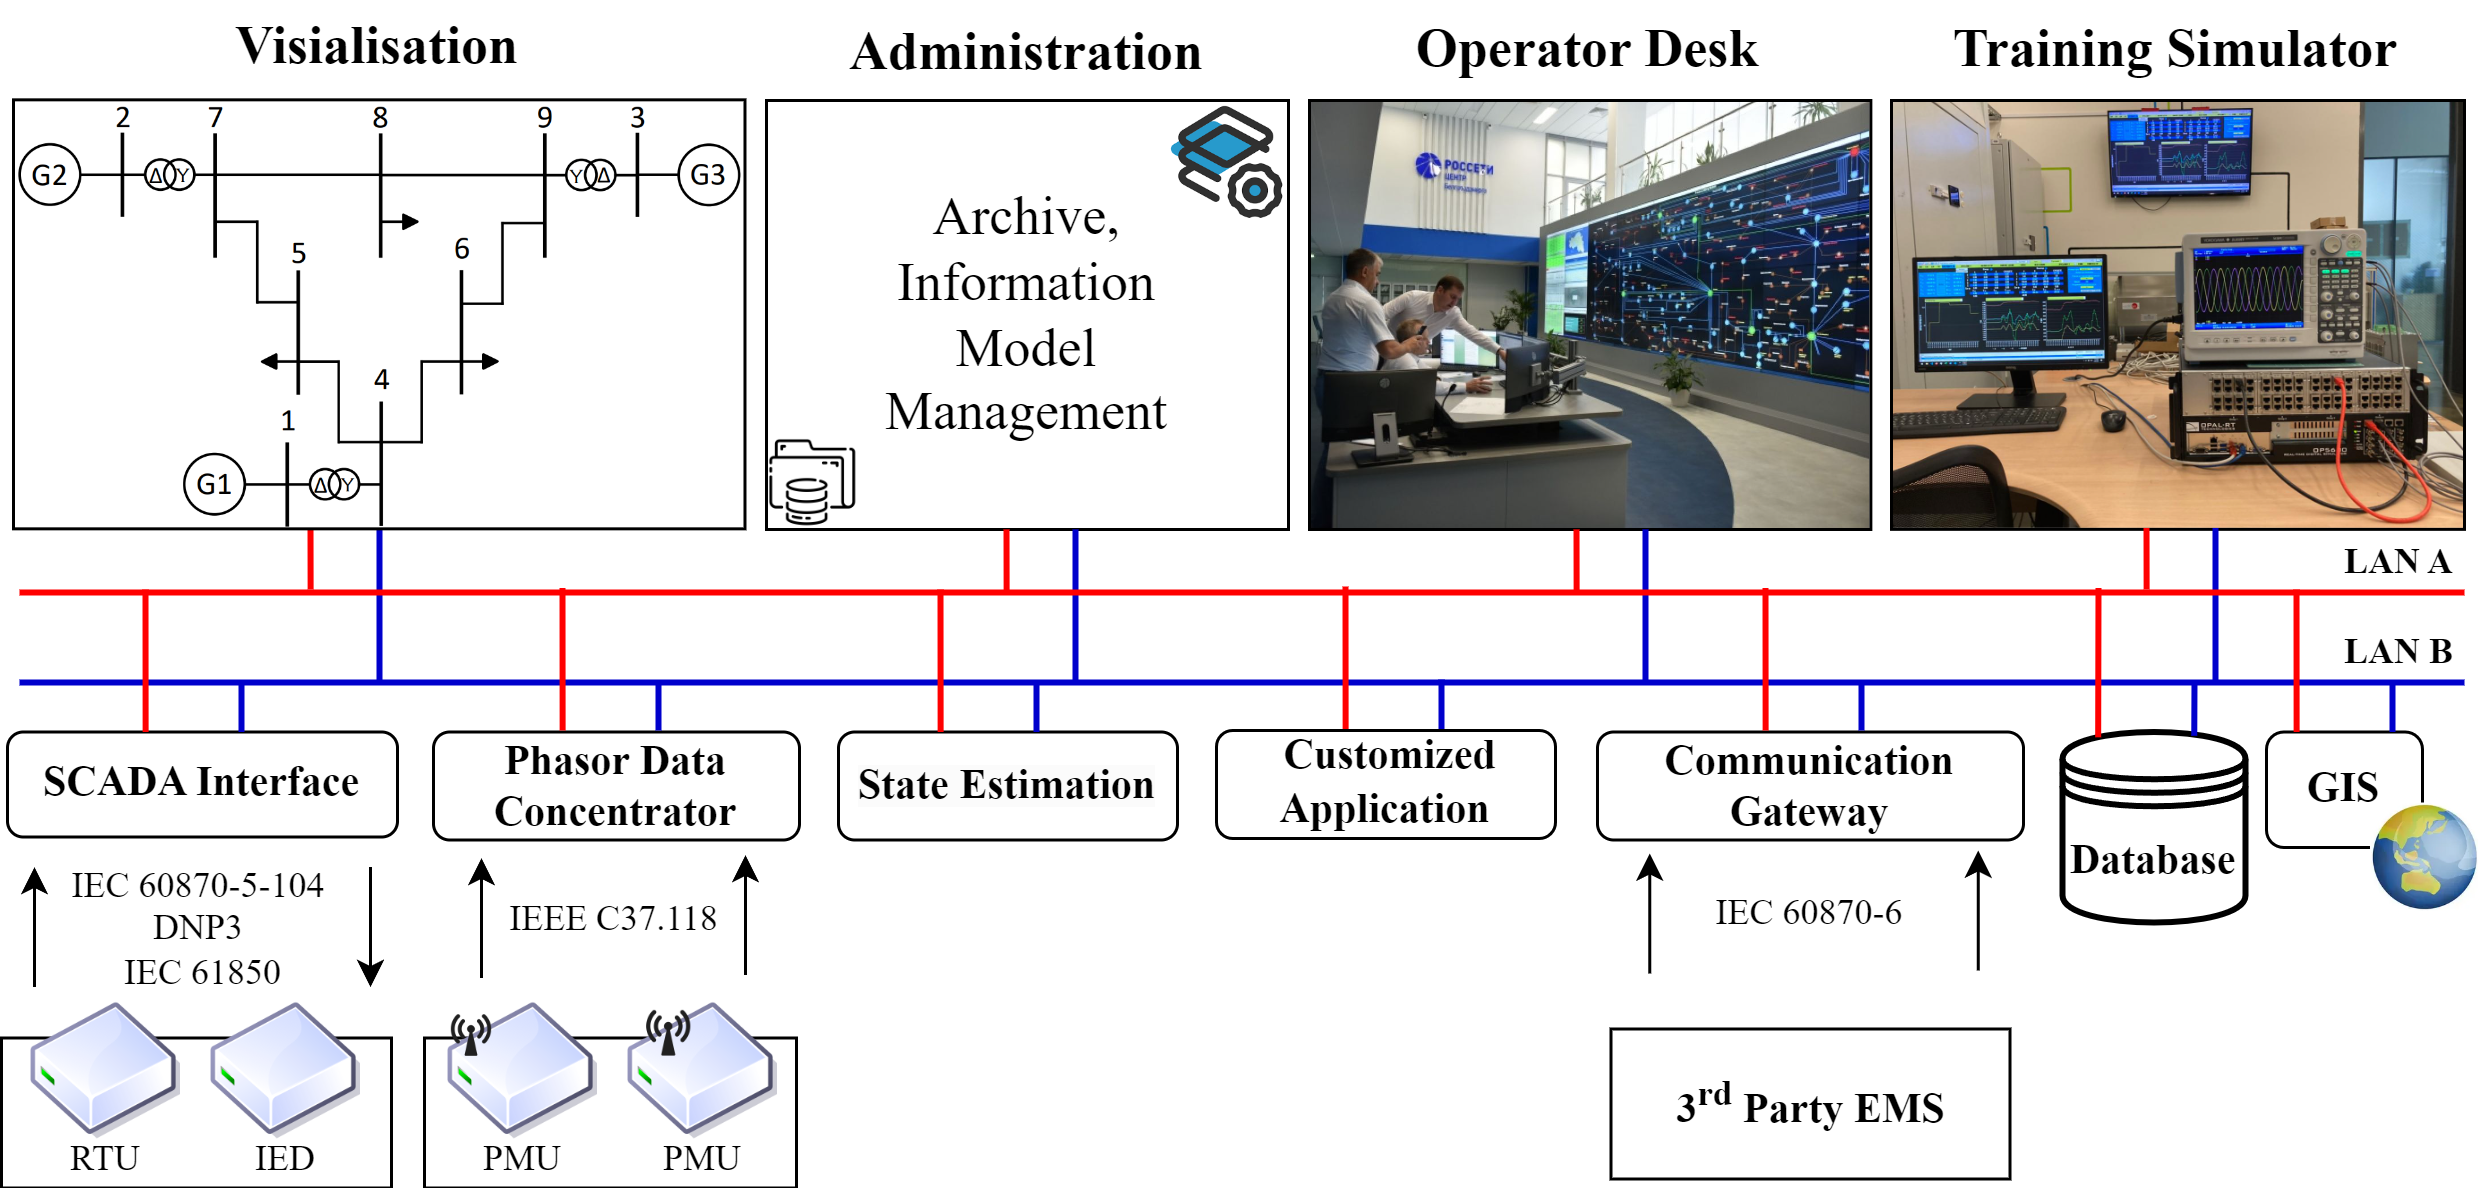
\includegraphics[width=1\textwidth]{ems_arch_2.png}
    \caption{Simplified EMS architecture.}
    \label{fig:ems_arch2}
\end{figure*}

The EMS primarily constitutes a front-end communication system responsible for data acquisition and control interactions, along with a critical Information Model Management (IMM) system. IMM contains a comprehensive topological model of the power system that details connectivity, component parameters, telemetry addresses, and telecontrol capabilities. Leveraging gathered telemetry data and the information model, the SE processes this information to yield a statistically robust and computable steady-state image of the power system's current operational state. Building upon the real-time state provided by the SE, the EMS incorporates a suite of secondary functions, also termed Advanced Decision and Optimization (ADO) functions. These applications provide essential model-based analyzes and decision support tools crucial for real-time operations and operational planning. Examples of these advanced functions include contingency screening, security assessment, switching simulations, and power flow optimization. 

\nomenclature{\(IMM\)}{Information Model Management}
\nomenclature{\(ADO\)}{Advanced Decision and Optimization }

ADO applications demand comprehensive topological information integrated with various operational degrees of freedom.  This includes predictions for load and generation, associated costs of generation, and reserves for generation. All of these factors contribute fundamentally to effectively accomplishing the intended optimization goals. Security assessment involves calculating short circuit current and protection security assessment (PSA) to evaluate protection settings, selectivity, and protection coordination of the system.

\nomenclature{\(PSA\)}{Protection Security Assessment}

Supporting these core functionalities are critical data management systems. This includes a historical data archive to store processed data, often compressed for long-term retention, and an immutable operational logbook that carefully documents all operator actions.
Access to EMS functionalities and visualized telemetry data is typically facilitated via workstation clients equipped with suitable Graphical User Interfaces (GUI). The overall control center EMS functional modules interactions visualized in Figure~\cref{fig:ems_modules_inter}.

\begin{figure*}[htbp]
    \centering
    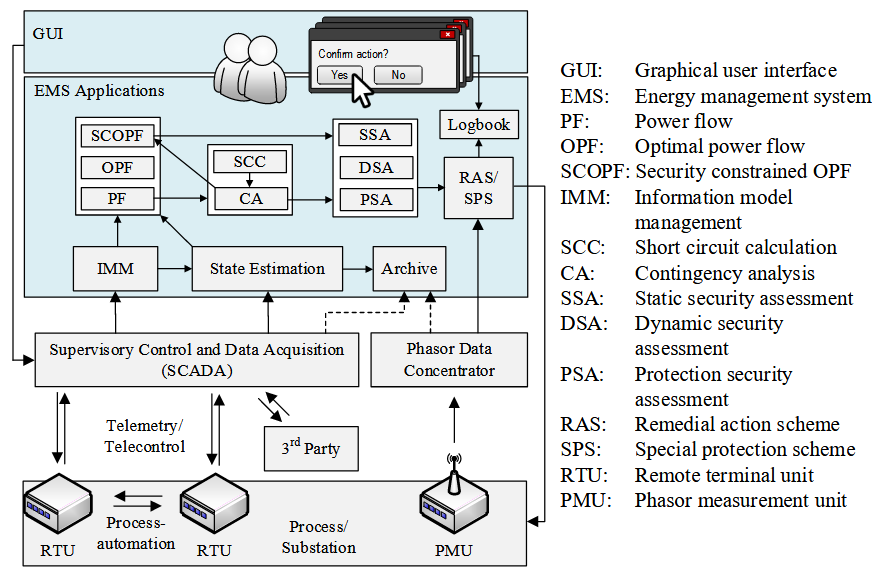
\includegraphics[width=1\textwidth]{ems_modules_interaction.png}
    \caption{Simplified EMS functional modules interaction  \autocite{8398846}.}
    \label{fig:ems_modules_inter}
\end{figure*}

Transmission systems benefit from extensive automation and real-time telemetry, while distribution systems, especially at medium- and low-voltage levels, face significant gaps in observability and controllability. This discrepancy arises from the historical design of distribution grids as passive networks, which now struggle to adapt to modern demands like renewable energy integration and real-time monitoring \autocite{8232008}.

\section{Measurement data}\label{sec:ch1/sec2}

SCADA systems and phasor measurement units (PMU) are two types of measurement systems that are commonly used for monitoring and control in power systems to ensure stability, reliability and efficiency. In general, it refers to the monitoring, control, and visualization of a technical process through computer systems that interact via an ICT network.

\nomenclature{\(PMU\)}{Phasor Measurement Units}

The integration of SCADA and PMU measurements enhances accuracy and reliability of state estimation. Although SCADA data are generally more accessible, PMU measurements offer higher accuracy and richer insights into the power system's status. SCADA measurements typically offer broad data on the power system's status, whereas PMU data provide precise insights at specific points. 

\subsection{Supervisory Control and Data Acquisition}\label{subsec:ch1/sec2/sub1}

SCADA is a combination of hardware and software used to gather real-time data from various components of the power grid. It enables operators to observe system performance, detect abnormalities, and take corrective actions either automatically or manually. SCADA typically integrates RTUs, IEDs, communication switches, merging units, programmable logic controllers (PLC), communication networks and human-machine interfaces (HMI) to maintain supervisory control over distributed assets \autocite{en12061084}. 

\nomenclature{\(PLC\)}{Programmable Logic Controller}
\nomenclature{\(HMI\)}{Human-Machine Interfaces}

The SCADA system's architecture generally comprises three key layers:
\begin{itemize}
    \item Field Layer: This level includes sensors, actuators, and devices such as RTUs, IEDs or PLCs, that collect operational data and perform local control actions.
    \item Communication Layer: Facilitates data transmission between field devices and control centers using wired or wireless networks.
    \item Control Center Layer: The central processing unit where HMIs, databases, and analytical tools are located. It is the operator's hub for system supervision and decision-making.
\end{itemize}
These layers work in coordination to provide a consistent view of the power system, allowing real-time management and historical analysis \autocite{nist_sp800_82}. In Figure~\cref{fig:scada_schematic} a SCADA system illustrated with structural components.

\begin{figure*}[htbp]
    \centering
    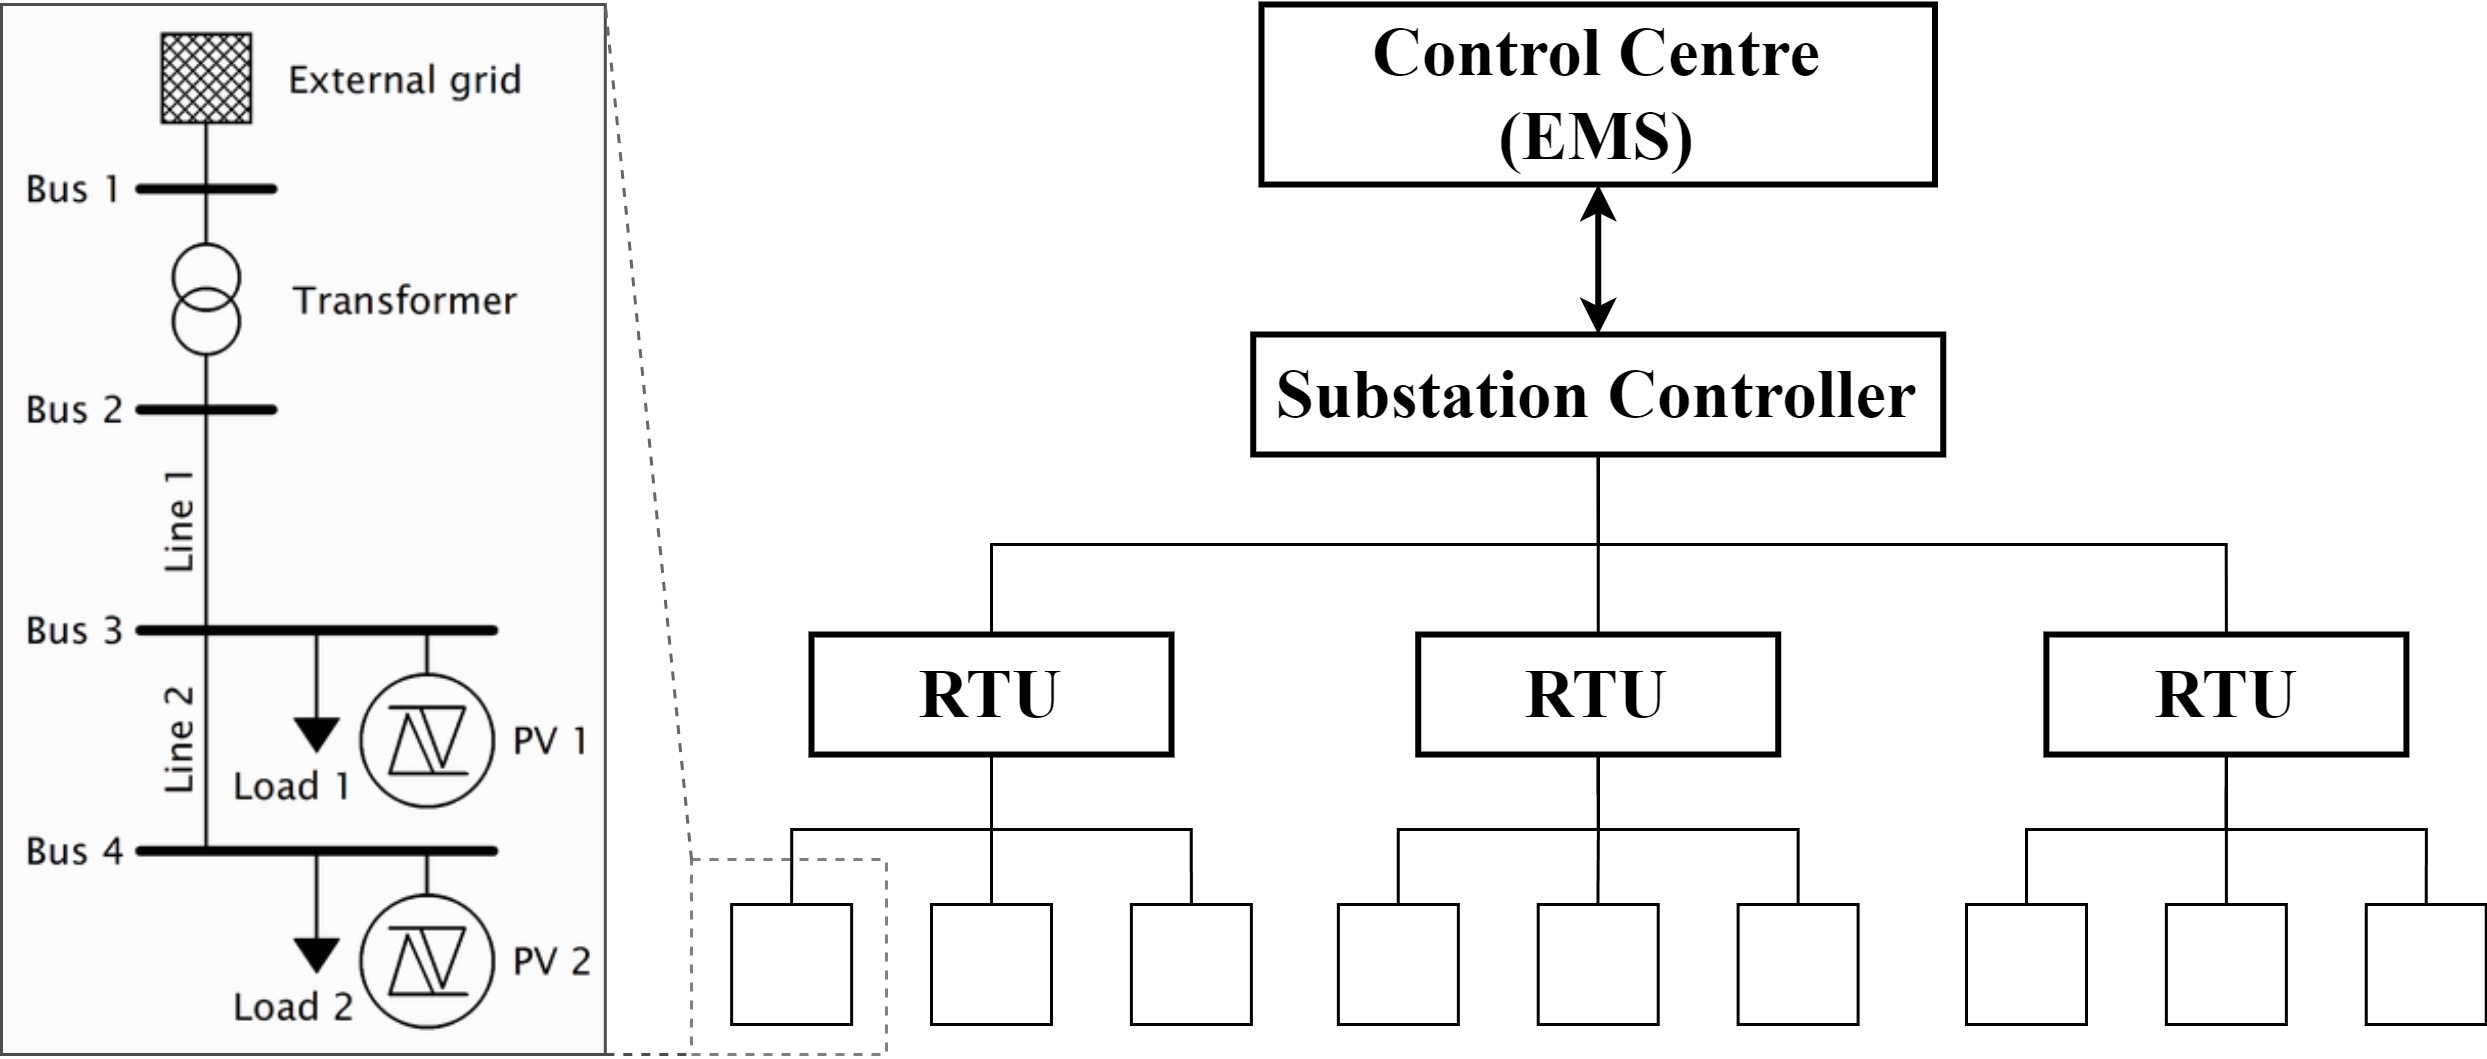
\includegraphics[width=1\textwidth]{scada_schematic2.png}
    \caption{Schematic representation of a SCADA system structure in a substation.}
    \label{fig:scada_schematic}
\end{figure*}

A modern SCADA system includes the following features:  
\begin{itemize}
    \item Real-Time Process Monitoring: Thanks to graphical visualizations and control panels, operators can immediately detect irregularities and respond quickly.
    \item Analytics and Optimization: Integrating machine learning modules and advanced analytics allow for predictive failure detection, more efficient resource management, and cost optimization.
    \item Scalability and Flexibility: Web-based SCADA solutions can be deployed in the cloud or on-premises, without limitations on the amount of process data or the number of users.
    \item Security and Easy Maintenance: Client-server architecture and use well-established encryption protocols (TLS, VPN), which greatly facilitates system protection and maintenance.
\end{itemize}

SCADA systems collect data from various sensors and devices in a power system, such as voltage and current sensors, circuit breakers and switchgear. Data transmission is realized via RTUs within substations through structured messages. 

These appear cyclically or triggered by event and contain the information itself, the cause of transmission and other relevant meta-data. The data rate depends on the device settings and the polling cycle. SCADA systems usually obtain new measurement sets every 1-10 seconds \autocite{1338122}.

Most communication occurs via fiber optic cables, whereas distribution networks frequently utilize ripple control or common telecommunication standards like LTE and GPRS for cost efficiency, as shown in Figure~\cref{fig:scada_communication}.

\begin{figure*}[htbp]
    \centering
    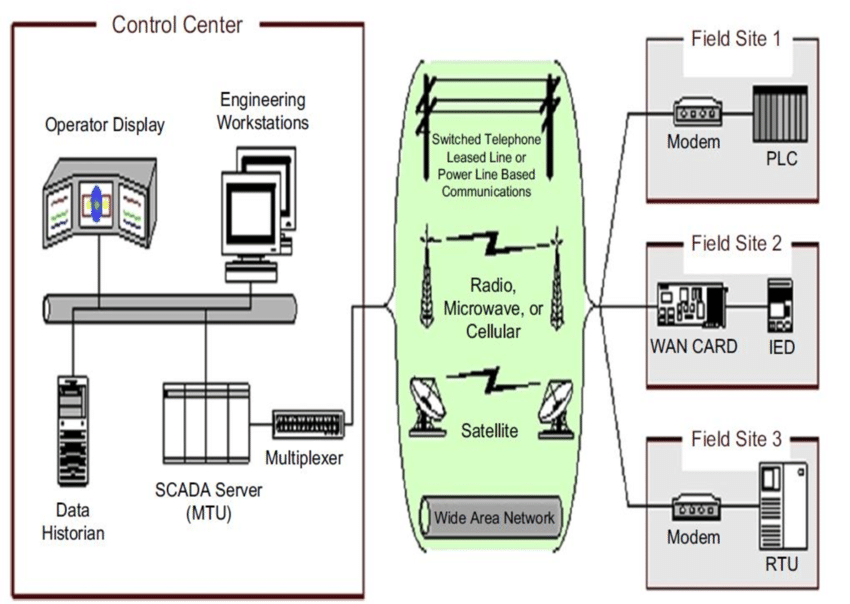
\includegraphics[width=0.8\textwidth]{scada_communication.png}
    \caption{SCADA System general layout communication system \autocite{nist_sp800_82}.}
    \label{fig:scada_communication}
\end{figure*}

Substations provide process information from field devices, which can be pre-processed and aggregated before transmission. Messages, measurements, and counts are timestamped and archived in the SCADA database. 

\subsection{Phasor Measurement Units}\label{subsec:ch1/sec2/sub2}

Phasors are complex numbers that represent the magnitude $X_m$  and phase angle $\varphi$ of a sinusoidal signal:
\begin{equation}
    x(t)=X_m \cos (\omega t+\varphi),
    % x(t)=\hat{x} \cos (\omega t+\varphi)
    \label{eq:phasor}
\end{equation}
as equivalent synchrophasor representation of the waveform:
\begin{equation}
    \begin{aligned}
X & =\left(X_{\mathrm{m}} / \sqrt{2}\right) \mathrm{e}^{\mathrm{j} \varphi} \\
& =\left(X_{\mathrm{m}} / \sqrt{2}\right)(\cos \varphi+\mathrm{j} \sin \varphi) \\
& =X_{\mathrm{r}}+\mathrm{j} X_{\mathrm{i}},
\end{aligned}
\end{equation}
where the magnitude is the rms value, $Xm /\sqrt{2}$, of the waveform and the subscripts $r$ and $i$ signify real and imaginary parts. The angle $\varphi$ is time-dependent, especially at $t = 0$. This phasor relates to angular frequency $\omega$; evaluations with other phasors must be done with the same time scale and frequency.

The required time synchronized phasor measurements are derived by PMUs, which are specialized devices that analyze the continuous analogue signals of AC voltage and current at a specific location in a power system and translate them into high-rate digital samples. Applying discrete Fourier transform, PMUs extract magnitude, phase, sequence, frequency, and rate of change of frequency (ROCOF), of the alternating signals given at its input terminal, as shown in Figure~\cref{fig:pmu_data}. Although PMU deployment is mainly in transmission systems, its use is increasingly expanding in distribution grids to improve observability \autocite{7779155}.

\nomenclature{\(ROCOF\)}{Rate of Change of Frequency}

\begin{figure*}[htbp]
    \centering
    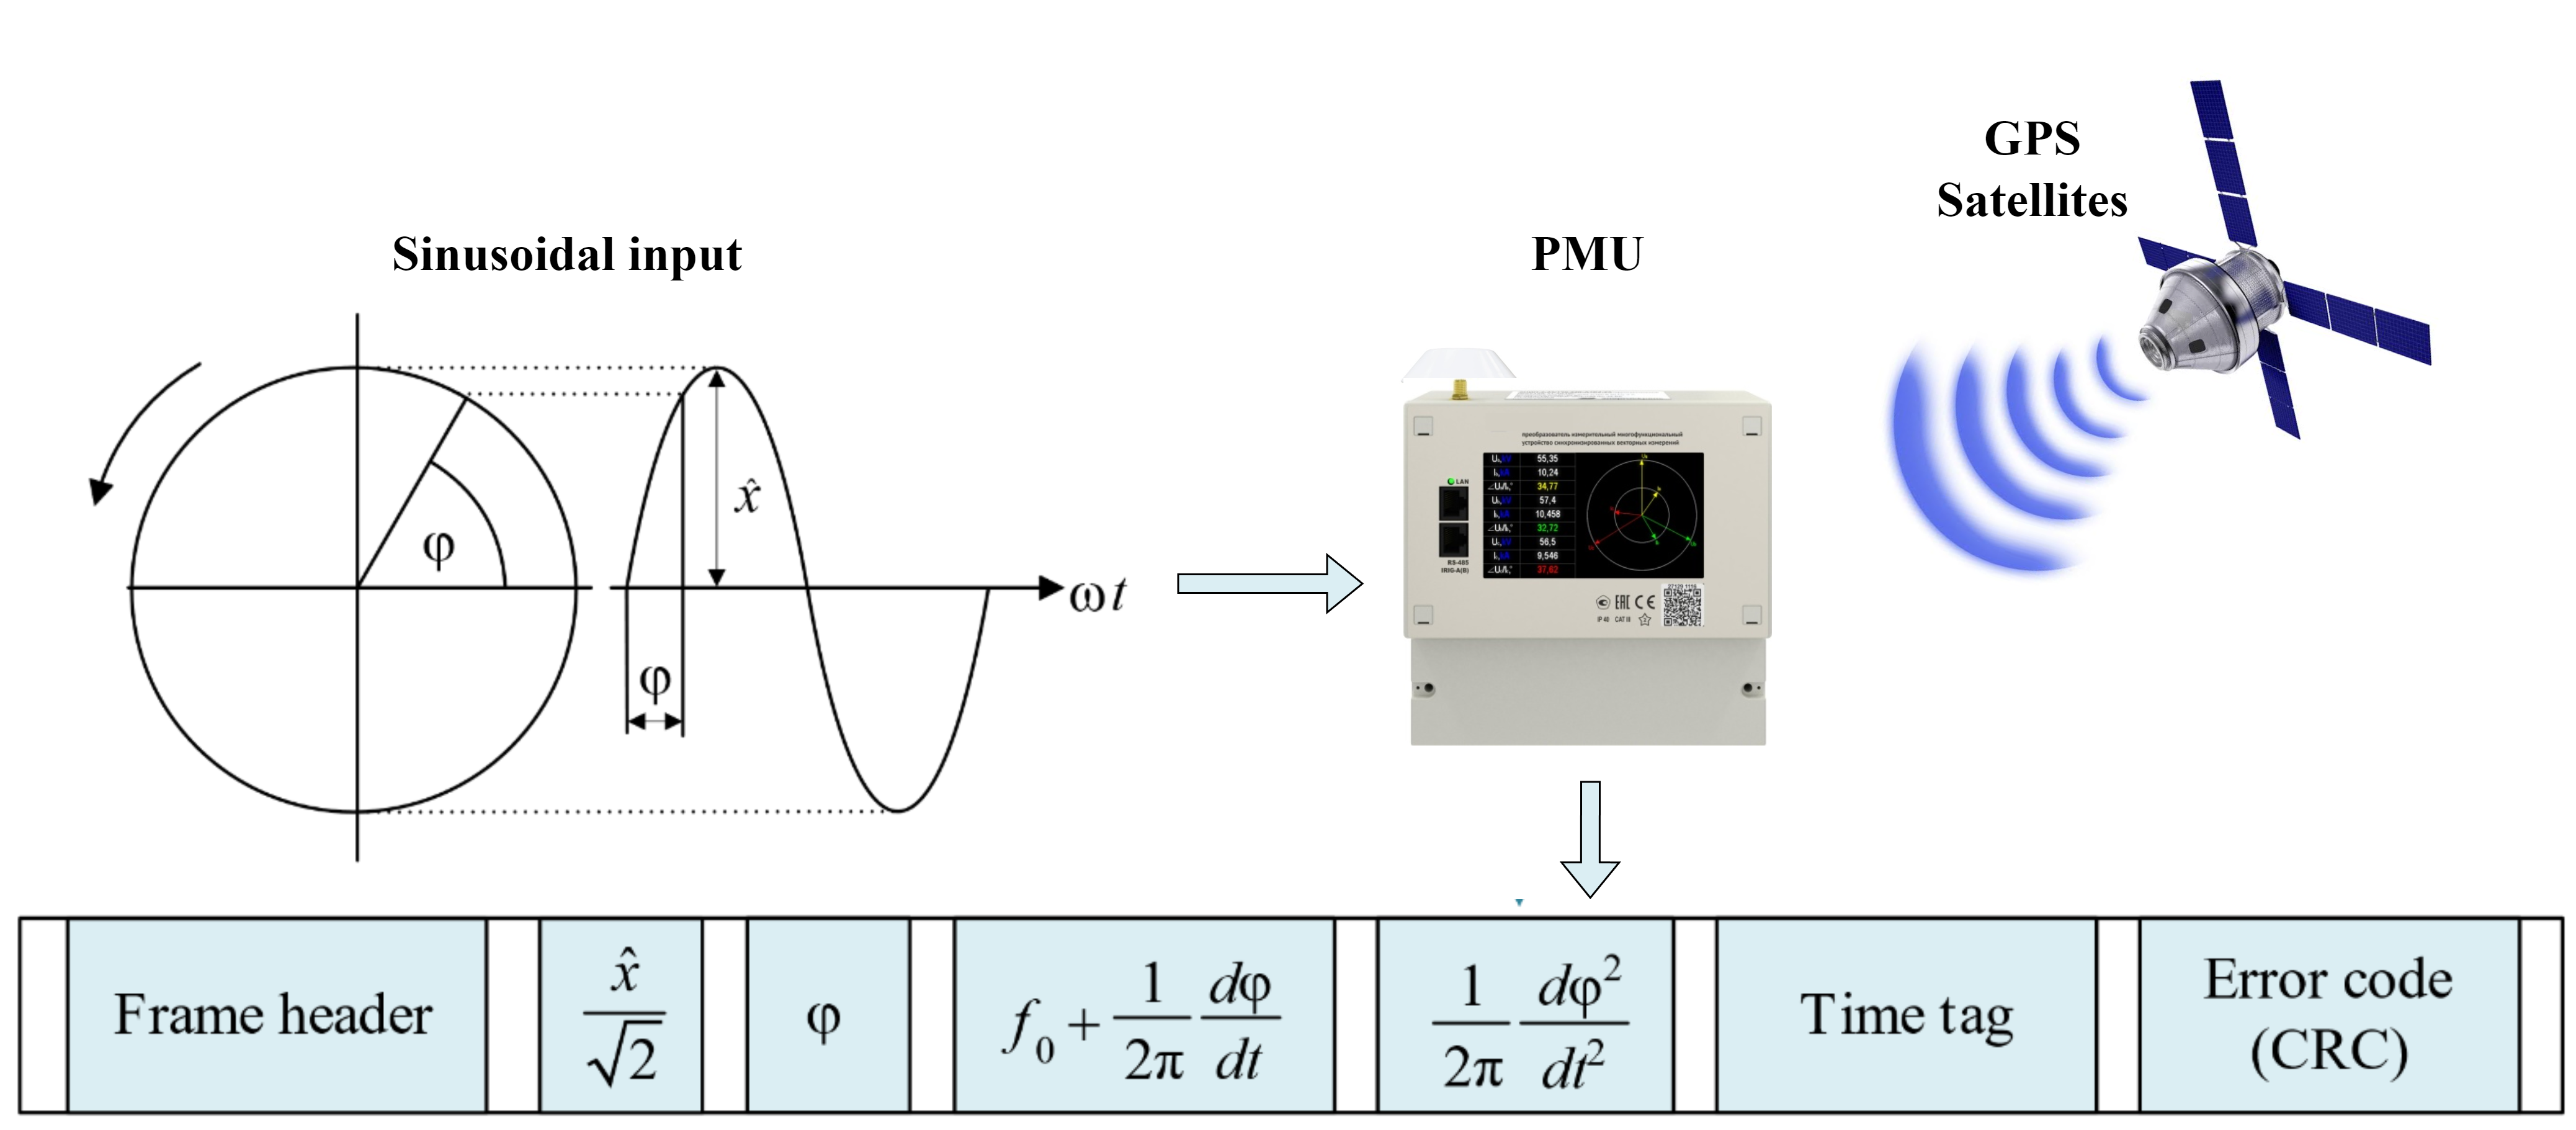
\includegraphics[width=1\textwidth]{pmu_data.png}
    \caption{The extraction of synchrophasor data packets in power systems.}
    \label{fig:pmu_data}
\end{figure*}

A PMU frame, in addition to measurement samples, includes a frame header with extra information such as cyclic redundancy check codes and measurement quality indicator \autocite{6111222}. A precise time source, such as Global Positioning System (GPS), provides the time signal to synchronize the measurements of various PMU devices.

Thanks to the precise time stamps provided by PMUs, applications for control, monitoring, and protection can access synchronized and comparable data streams in real time \autocite{5447627}. Commercial PMUs support a broad range of reporting rate, from 10 $reports/sec$ up to 240 $reports/sec$. The time tag accuracy requirement is $\pm1\mu s$, which corresponds to an angle error of 0.018 degrees for a 50 $Hz$ system.

\section{Power System State Estimation}\label{sec:ch1/sec3}

Due to the presence of noise, communication latency, missing measurements, and temporary communication failures, the raw telemetered data obtained from acquisition are often incomplete and have potential for errors. In practice, the measurements collected - such as bus voltage magnitudes, injected active and reactive power at buses, and power flows along branches - are inherently imperfect, affected by instrument inaccuracies, data conversion errors, communication noise, and occasional data corruption. Additionally, due to redundancy in measurement placement and sporadic data availability, the system may be partially unobservable at any given time.

To address these issues, state estimation algorithms are employed to:
\begin{itemize}
    \item Compensate for measurement noise and inaccuracies.
    \item Interpolate missing data.
    \item Detect and suppress bad data.
    \item Ensure observability in the presence of incomplete datasets.
    \item Generate a consistent and physically feasible system state.
\end{itemize}

To realize these functionality, the typical structural modules of SE is applied in diagram and presented in Figure~\cref{fig:se_flowchart}. To maintain an accurate system representation, the topology-processor \autocite{32475}, a specialized block within the state estimator, is continuously informed of any alterations in the network's structure and the most recent state assessments, allowing it to dynamically revise the network map. Based on this current topological understanding and the incoming stream of measurements, the system then performs an observability analysis to determine if the measurement set is rich enough to fully characterize the network's state. Only after the network's topology and its observability are adequately determined, the state estimator can proceed with its core task: calculating the optimal state vector from the available measurements and the underlying network model. 

\begin{figure*}[htbp]
    \centering
    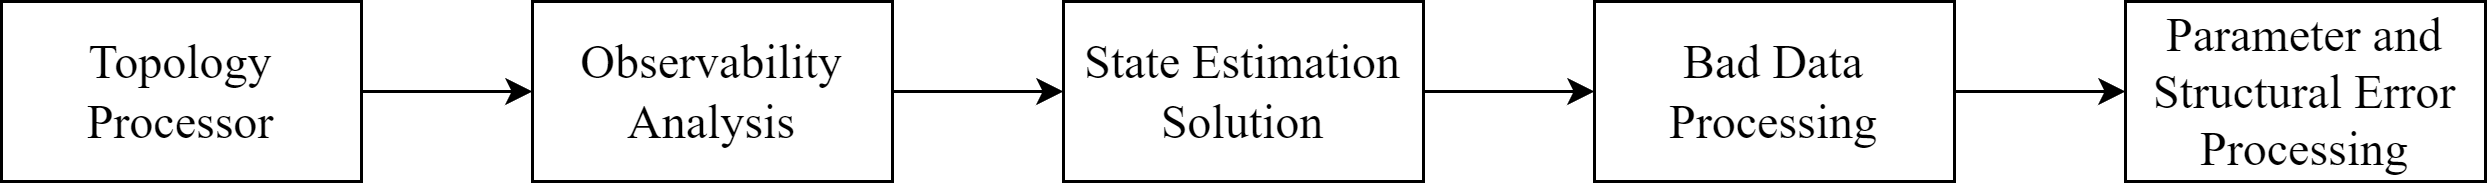
\includegraphics[width=1\textwidth]{se_flowchart.png}
    \caption{State Estimation functional modules.}
    \label{fig:se_flowchart}
\end{figure*}

Among the algorithmic part of SE the weighted least squares method has become a de facto standard to approximate a steady-state representation of the power system \autocite{abur2004power}. However, least squares SE algorithm is not very robust against  measurement outliers or large deviations \autocite{WU199080}, which caused such a factors as:
\begin{itemize}
    \item Sensor errors: Sensors may introduce measurement errors due to factors like manufacturing defects, environmental factors, and aging.
    \item Communication errors: Sensors transmit measurements to the state estimator through communication channels. Various factors, including channel noise, interference, and cyber-attacks, can cause errors in these transmitted measurements.
    \item Environmental factors: Environmental factors like temperature, humidity, and vibration can cause measurement errors.
    \item Human errors: Measurement inaccuracies can arise from human mistakes during sensor installation, calibration, and operation.
\end{itemize}

Thus, an essential next step is to apply thorough bad data detection and diagnostic procedures to identify inaccuracies in system parameters and the structural model. For doing that, a detailed database of electrical equipment characteristics and types for establishing a precise network model must be established. In addition, a covariance matrix with estimated measurement error variances is necessary.

Spreading of synchrophasor technology within PMUs gave an impetus to development of linear and hybrid state estimators evolved \autocite{1717598, BI20081343, 6878488}. In case of a high number of PMUs, the system could become completely observable. The direct measurement of the state variables on all buses allows a simple and fast linear SE solution \autocite{8620530}. The calculation time for large SE problems can be reduced by applying hierarchical or distributed SE schemes \autocite{7182780, 4162601}.

Due to the constantly evolving nature of power systems, it is essential to monitor their dynamic behavior in real time. This requires performing state estimation at short intervals. Traditional static state estimators fall short in accurately capturing these rapid changes, especially in PEDGs. To address this limitation, a technique known as Dynamic State Estimation (DSE) has been developed \autocite{1099844, 4074246}. DSE leverages a physical model that reflects the time-varying characteristics of the power system, enabling it to forecast the system's state at the next time step $(t+1)$ based on information from the current step $(t)$. One of the key benefits of DSE is its predictive capability, which allows for proactive decision-making. This forecasting feature significantly enhances the effectiveness of energy management system operations and control strategies.

\nomenclature{\(DSE\)}{Dynamic State Estimation}

To detect and identify issues like bad data, network reconfigurations, and abrupt state variations in DSE is suggested in \autocite{Nishiya1982}. Utilizing simple dynamic state vector models and linearized measurement equations, Kalman filtering theory is employed for estimation \autocite{Leite1983}, with one of the most widely used methods in power system DSE being the Extended Kalman Filter (EKF), which considers both the incoming measurements and the predicted state to obtain an optimal estimate of the system state, as mentioned in \autocite{Mandal1995}.

The study in \autocite{4510059} thoroughly examines the use of EKF to incorporate dynamic state variables, such as generator rotor speed and angle, into SE. This EKF-based process is validated on a multi-machine system under different disturbances. EKF-UI, an extension, is used in \autocite{5871327} for joint estimation of states and unknown inputs in synchronous machines. In \autocite{6024863}, a new distributed EKF framework is introduced, addressing the complexities of large-scale renewables and smart grids. This method enhances computational speed by dividing systems into subsystems for distributed implementation of DSE in extensive power networks.

The EKF, a commonly used estimation algorithm for nonlinear systems, faces challenges like implementation difficulty, tuning complexity, and limited reliability to nearly linear systems within update intervals \autocite{1271397}. To address EKF's issues due to linearization, the Unscented Transformation (UT) was developed to propagate mean and covariance through nonlinear transformations. The benefits of the Unscented Kalman Filter (UKF), rooted in UT, are discussed in literature \autocite{Valverde2011, 6019414, 6112697}. Studies \autocite{5619951, 6112697} confirm UKF's superior accuracy and easier application for generator dynamics with simulations. Analysis with three power systems demonstrates UKF's superior filtering over EKF in slower dynamic changes \autocite{Valverde2011}. UKF's effectiveness in estimating frequency, amplitude, and phase, even in noisy conditions, is shown in \autocite{6019414}. A non-derivative Kalman filtering approach for nonlinear systems control is explored in \autocite{5892889}, and a new state estimation method using UKF for power and frequency is detailed in \autocite{6142065}.

\nomenclature{\(EKF\)}{Extended Kalman Filter}
\nomenclature{\(UKF\)}{Unscented Kalman Filter}

Though hybrid, linear, and DSE techniques are frequently explored in research, their adoption in operational EMS settings remains limited due to their strong reliance on dependable ICT \autocite{8624411}. Literature proposes algorithms to enhance DSE speed and robustness \autocite{7742899,WANG2020105390,8063917,7864445}, and for advanced uses like model predictive control \autocite{5342446, 6632979}, online DSA \autocite{SUN2016160, 6158623}, and wide area control \autocite{6202751}. However, detailed plans for the next-generation EMS and its future-proof architecture incorporating DSE for system operations are still lacking. The primary distinctions between SSE and DSE lie in their applications, modeling, and data needs. SSE is used for dispatching and monitoring voltage and flow limit breaches, while DSE is relevant to DSA and time-domain model calibration. Most power system DSE techniques employ Kalman filters, which typically rely on data streams from PMU-based WAMS \autocite{6802979,5871327,7501856,TEBIANIAN2015109}. General overviews of DSE algorithms and applications are found in \autocite{Simon_2006,Singh_Pal_2019}, with power system-specific DSE algorithms assessed in \autocite{6887334}. Table \ref{tab:se_comparison} compares the previously discussed state estimation methods.

% Please add the following required packages to your document preamble:
\begin{table}[]
\caption{Comparison of state estimation approaches}
\label{tab:se_comparison}
\resizebox{\textwidth}{!}{%
\begin{tabular}{|l|llll|}
\hline
\multicolumn{1}{|c|}{\multirow{2}{*}{\textbf{}}} & \multicolumn{4}{c|}{\textbf{State Estimation Type}} \\ \cline{2-5} 
\multicolumn{1}{|c|}{} & \multicolumn{1}{c|}{\textbf{Classic}} & \multicolumn{1}{c|}{\textbf{Hybrid}} & \multicolumn{1}{c|}{\textbf{Linear}} & \multicolumn{1}{c|}{\textbf{Dynamic}} \\ \hline
\textbf{\begin{tabular}[c]{@{}l@{}}Data \\ source\end{tabular}} & \multicolumn{1}{c|}{SCADA} & \multicolumn{1}{c|}{SCADA and PMU} & \multicolumn{1}{c|}{PMU} & \multicolumn{1}{c|}{PMU} \\ \hline
\textbf{\begin{tabular}[c]{@{}l@{}}Model \\ basis\end{tabular}} & \multicolumn{1}{c|}{\begin{tabular}[c]{@{}c@{}}Algebraic steady \\ state power flow\end{tabular}} & \multicolumn{1}{c|}{\begin{tabular}[c]{@{}c@{}}Algebraic steady \\ state power flow\end{tabular}} & \multicolumn{1}{c|}{\begin{tabular}[c]{@{}c@{}}Algebraic dynamic \\ power flow\end{tabular}} & \begin{tabular}[c]{@{}l@{}}Differential-algebraic \\ equation-based \\ time domain model\end{tabular} \\ \hline
\textbf{\begin{tabular}[c]{@{}l@{}}Input \\ data\end{tabular}} & \multicolumn{1}{l|}{\begin{tabular}[c]{@{}l@{}}Bus voltage \\ magnitudes: $U_{i,j}$;\\ Bus injections:  \\ $P_{i,j}, Q_{i,j}, I_{ij}$;\\ Branch admittance: \\ $Y = G_{ij},+jB_{ij}$;\end{tabular}} & \multicolumn{1}{l|}{\begin{tabular}[c]{@{}l@{}}Bus voltage \\ magnitudes $U_{i,j}$;\\ selected $U(t)$;\\ Bus injections  \\ $P_{i,j} Q_{i,j}$;\\ Branch flows \\ $P_{ij}, Q_{ij}, I_{ij}$;\\ Branch admittance  \\ $Y = G_{ij},+jB_{ij}$\end{tabular}} & \multicolumn{1}{l|}{\begin{tabular}[c]{@{}l@{}}Complex bus \\ voltages $U_{i,j}(t)$;\\ Branch admittance  \\ Y = $G_{ij},+jB_{ij}$\end{tabular}} & \begin{tabular}[c]{@{}l@{}}Complex bus \\ voltages $Ui,j(t)$; \\ Branch currents $I(t)$; \\ Parameter set \\ for equipment \\ and controller models\end{tabular} \\ \hline
\textbf{\begin{tabular}[c]{@{}l@{}}Resulting \\ state \\ variables\end{tabular}} & \multicolumn{1}{l|}{\begin{tabular}[c]{@{}l@{}}$U_{i,j}$, branch flows, \\ transformer tap \\ positions, \\ switching state \\ (corrected topology)\end{tabular}} & \multicolumn{1}{l|}{$U_{i,j}$, branch flows} & \multicolumn{1}{l|}{\begin{tabular}[c]{@{}l@{}}$U_{i,j}$, branch flows, \\ topology\end{tabular}} & \begin{tabular}[c]{@{}l@{}}Algebraic states: \\ {[}$z_1,...,z_n${]}, \\ differential states: \\ {[}$x_1,...,x_n${]},\\ and state derivatives: \\ {[}$\dot{x}_1,...,\dot{x}_n${]}\end{tabular} \\ \hline
\textbf{\begin{tabular}[c]{@{}l@{}}Complexity \\ and \\ computing \\ time\end{tabular}} & \multicolumn{1}{l|}{Medium} & \multicolumn{1}{l|}{Medium} & \multicolumn{1}{l|}{Low} & High \\ \hline
\textbf{\begin{tabular}[c]{@{}l@{}}Complexity \\ and \\ computing \\ time\end{tabular}} & \multicolumn{1}{l|}{Medium} & \multicolumn{1}{l|}{Medium} & \multicolumn{1}{l|}{Low} & High \\ \hline
\textbf{\begin{tabular}[c]{@{}l@{}}EMS \\ implementation\end{tabular}} & \multicolumn{1}{l|}{State of the art} & \multicolumn{1}{l|}{\begin{tabular}[c]{@{}l@{}}Some \\ implementations\end{tabular}} & \multicolumn{1}{l|}{Applied by WAMS} & \begin{tabular}[c]{@{}l@{}}Scarce implementations, \\ experimental state\end{tabular} \\ \hline
\end{tabular}%
}
\end{table}

\section{Static State Estimation}\label{sec:ch1/sec4}

Static state estimation (SSE) is defined as the process for determining the voltage magnitudes and angles of all buses in the power system at a given time, under the assumption of steady-state operation \autocite{Phadke12008springer}. This method is based on the quasi-static nature of power systems, where system changes are relatively slow compared to the SE time scale. It has served as a cornerstone of modern power network control systems since its introduction in the early 1970s by Schweppe and Handschin \autocite{4074022}. 

\nomenclature{\(SSE\)}{Static State Estimation}

\subsection{Maximum likelihood method}\label{subsec:ch1/sec4/sub1}
% \subsubsection{Maximum likelihood method}

Maximum likelihood estimation (MLE) is a statistical technique used to estimate the parameters of a model by selecting the values that make the observed data most probable. The principle behind MLE is to identify the set of parameters that maximizes the likelihood function, which quantifies how well the model explains the measured data. In the context of power system state estimation, this involves modeling measurement errors, typically assumed to follow a normal distribution, and then deriving the parameter values that best align the model with the data. The likelihood function is based on the joint probability of the measurements given the state variables, and the estimation process seeks to find the state that maximizes this function. 

\nomenclature{\(MLE\)}{Maximum Likelihood Estimation}

Measurement errors are typically assumed to follow a Normal distribution, characterized by two parameters: the mean $\mu$ and the variance $\sigma^2$. The normal probability density function (PDF) for a random variable $z$, with mean $\mu$, and standard deviation $\sigma$ can be defined as \autocite{Abur2004}:

\nomenclature{\(PDF\)}{Probability Density Function}

\begin{equation}
    f(z)=\frac{1}{\sqrt{2 \pi} \sigma} \exp \left[-\frac{1}{2 \sigma^{2}}\left(z-\mu\right)^{2}\right].
\end{equation}

Taking into account the assumption based on considering m independent measurements and each having the same Gaussian PDF, and each measurement is assumed to be independent of the others, the joint pdf can be simply written as the product of individual PDFs. The resulting  product function $f_m(z)$ can be given by:

\begin{equation}
    f_{m}(z)=f\left(z_{1}\right) f\left(z_{2}\right) \ldots f\left(z_{m}\right).
\end{equation}

The function $f_m(z)$ is called the likelihood function for the set of $m$ measurements. It measures the probability of observing measurements in vector $z$. Maximum likelihood estimation of $f_m(z)$ involves maximizing it by varying parameters $\mu$ and $\sigma$ of the density function. This is simplified by maximizing the logarithm of the likelihood function, with its value given by function $f(z)$:

\begin{equation}
    \log f(z)=-\frac{1}{2} \frac{(z-\mu)^{2}}{\sigma}-\log \sigma \sqrt{2 \pi},
\end{equation}
or the modified function \(L=\log f_{m}(z)\).

\begin{equation}
    L=\sum_{i=1}^{m} \log f\left(z_{i}\right)=-\sum_{i=1}^{m} \log \sigma_{i}-\frac{m}{2} \log 2 \pi-\frac{1}{2} \sum_{i=1}^{m}\left(\frac{z_{i}-\mu_{i}}{\sigma_{i}}\right)^{2}.
\end{equation}

The maximum likelihood estimate is obtained by finding the maximum of \(\log f_{m}(z)\), which can also be obtained by finding the minimum of 

\begin{equation}
    \min J(z)=\sum_{i=1}^{m}\left(\frac{z_{i}-\mu_{i}}{\sigma_{i}}\right)^{2},
\label{eq:wls_estimator}    
\end{equation}
which is known as \textit{weighted least squares} estimator.

The minimization problem can be rewritten, considering the form of residuals \(r_{i}=z_{i}-\mu_{i}\), if $r_i$ is residual of measurement $i$. Here, the mean $\mu_{i}$, which is the expected value of $z_{i}$, can be expressed as $h_i(x)$, a nonlinear function relating the system state vector $x$ to the $i$th measurement. Considering that the square of residual $r_i$ weighted by $W_i$ is equal to inverse of error variance $\sigma_{i}^2$, the minimization problem can also be written as

\begin{equation}
    \begin{array}{c}
    \operatorname{min} \quad \sum_{i=1}^{m} W_{i} r_{i}^{2}, \\
    \text { s.t. } z_{i}=h_{i}(x)+r_{i}, i=1, \ldots, m.
\end{array}
\label{eq:min_rsd}
\end{equation}

In case of matrix format of the above equations:

\begin{equation}
    \begin{array}{l}
\min J(x)=[z-h(x)]^{T} [z-h(x)] / R_{ii},
\end{array}
\end{equation}
where
\begin{equation}
    R=\left[\begin{array}{llll}
\sigma_{1}^{2} & & & \\
& \sigma_{2}^{2} & & \\
& & \ddots & \\
& & & \sigma_{m}^{2}
\end{array}\right],
\label{eq:mlm_r}
\end{equation}
where $[R]$ is the \textit{covariance matrix} of measurement errors.

To address this optimization problem, the solution is required to follow the first-order optimality condition, which:
\begin{equation}
    \frac{\partial J}{\partial x}=0 \quad \rightarrow \quad\left[-\frac{\partial h}{\partial x}\right]^{T} R^{-1}[z-h(x)]=0,
    \label{eq:mlm_optcond}
\end{equation}
where \(H(x)=\delta h / \delta x\) is the Jacobian matrix of dimension (m × n) measurement.

As $h(x)$ in AC SE is nonlinear, Gauss-Newton method can be applied to linearize the function. Considering \(g(x)=\frac{\partial J}{\partial x}\) and expanding $g(x)$ around the state vector $x^k$ the following iterative procedure can be obtained:
\begin{equation}
    h(x+\Delta x) \approx h(x)+H(x) \Delta x,
\end{equation}

\begin{equation}
    x^{k+1}=x^{k}-\left[G\left(x^{k}\right)\right]^{-1} g\left(x^{k}\right),
\end{equation}

\begin{equation}
    G\left(x^{k}\right)=\frac{\partial g\left(x^{k}\right)}{\partial x}=H^{T}\left(x^{k}\right) R^{-1} H\left(x^{k}\right),
\end{equation}

\begin{equation}
    g\left(x^{k}\right)=-H^{T}\left(x^{k}\right) R^{-1}\left(z-h\left(x^{k}\right)\right.,
\end{equation}
where symmetric matrix \(H^{T}\left(x^{k}\right) R^{-1} H\left(x^{k}\right)=G(x)\) is  called the gain matrix, $k$ is the iteration index, $x^k$ is the solution vector at iteration $k$.

\subsection{Network Topology}\label{subsec:ch1/sec4/sub2}
% \subsubsection{Network topology}
The implementation of SE requires detailed information about network topology and parameters. The component model that represents the entire network presented by: tap changing and phase shifting transformer, transmission line (TL), shunt capacitors or reactors and loads with generators.  

\nomenclature{\(TL\)}{Transmission Line}

\textbf{Transmission line}. A two port $\pi$-model is utilized to characterize the positive sequence of the TL. It is assumed that the power system is operating in steady state mode and under balanced condition. This requires that all TLs are fully transposed, all bus loads and branch power flows will be three phase and balanced,  and all other series or shunt devices will be symmetrical in the three phases. The transmission line with a positive sequence series impedance of \(R + jX\) and total line charging susceptance of $j2B$ can be presented as equivalent circuit presented, shown in Figure~\cref{fig:pi_model}.

\begin{figure}[htbp]
    \centering
    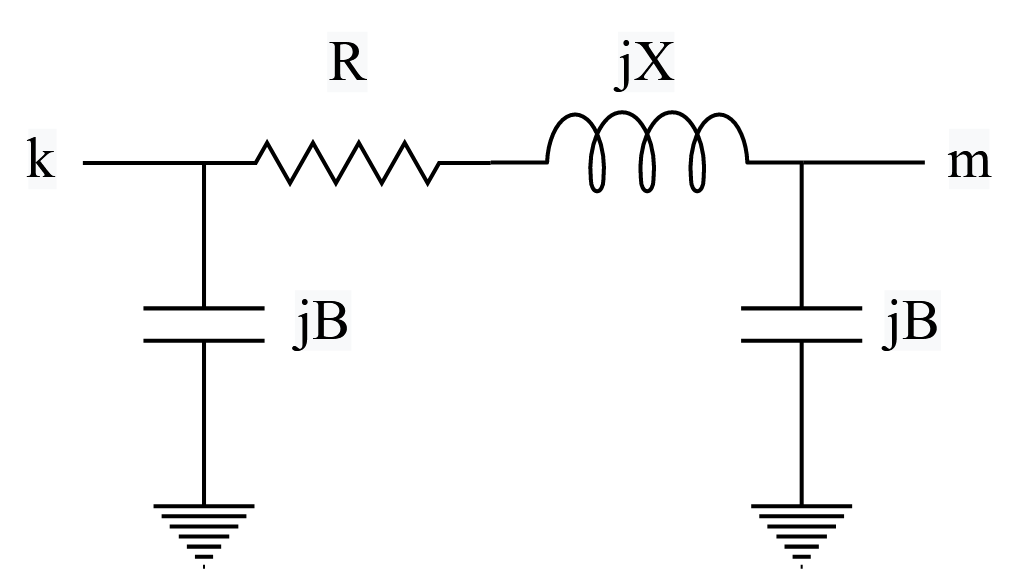
\includegraphics[width=0.45\linewidth]{pi_model.png}
    \caption{Two port $\pi$-model equivalent circuit of TL.}
    \label{fig:pi_model}
\end{figure}

\textbf{Tap Changing Transformer}. Transformers can be modeled as ideal transformer in series with resistance and inductance, with terminal buses $m$ and $k$ on impedance side and the tap side bus respectively, as shown in Figure~\cref{fig:tf_eqc}.

\begin{figure}[htbp]
    \centering
    
\includegraphics[width=0.8\linewidth]{TF_EQC.png}
    \caption{Equivalent circuit of tap changing transformer.}
    \label{fig:tf_eqc}
\end{figure}

The nodal equations for the two-port circuit in Figure~\cref{fig:tf_eqc} are obtained by expressing the currents $i_{lm}$ and $i_{m}$ at the ends of the series branch \(R+jX\). If $y$ is the branch admittance \(l-m\), the terminal current injections are described by:
\begin{equation}
    \left[\begin{array}{c}
i_{\ell m} \\
i_{m}
\end{array}\right]=\left[\begin{array}{rr}
y & -y \\
-y & y
\end{array}\right]\left[\begin{array}{c}
v_{\ell} \\
v_{m}
\end{array}\right]
\end{equation}
Substituting for \(i_{lm} = a \cdot i_{k}\) and \(v_{l} = v_{k}/a\), the following form will be obtained:
\begin{equation}
    \left[\begin{array}{c}
i_{k} \\
i_{m}
\end{array}\right]=\left[\begin{array}{rr}
y / a^{2} & -y / a \\
-y / a & y
\end{array}\right]\left[\begin{array}{c}
v_{k} \\
v_{m}
\end{array}\right]
\end{equation}
where $a$ is the in phase tap ratio.

\textbf{Shunt Capacitors or Reactors}. To manage voltage or reactive power, installing shunt capacitors or reactors is an option. The sign of the susceptance indicates the type: negative for capacitors and positive for reactors.

\textbf{Loads and Generators}. Power injections from loads and generators, expressed as complex power, remain independent of the network model. In contrast, constant impedance loads are accounted for as shunt admittances at respective buses.

\textbf{Network Modeling}. Mentioned component models are utilized to construct a complete power system model. This involves formulating equations for each node based on Kirchhoff's current law, as follows:
\begin{equation}
    I=\left[\begin{array}{c}
i_{1} \\
i_{2} \\
\vdots \\
i_{N}
\end{array}\right]=\left[\begin{array}{cccc}
Y_{11} & Y_{12} & \cdots & Y_{1 N} \\
Y_{21} & Y_{22} & \cdots & Y_{2 N} \\
\vdots & \vdots & \vdots & \vdots \\
Y_{N 1} & Y_{N 2} & \cdots & Y_{N N}
\end{array}\right]\left[\begin{array}{c}
v_{1} \\
v_{2} \\
\vdots \\
v_{N}
\end{array}\right]=Y \cdot V
\end{equation}
where \\ 
$I$ is the net current injection phasors vector\\
$V$ is the bus voltage phasors vector\\  
$Y_{km}$ is the ($k,m$)th element of the $Y$ matrix\\ 
$N$ is the number of bus\\
$i_k$ is the current injection phasor in bus $k$\\
$v_k$ is the voltage at bus $k$

\textbf{Measurement Model}. The SE of the power system usually involves measurements such as line power flows, bus power injections, and bus voltage magnitudes, represented using either rectangular or polar coordinates. For a system of $N$ buses, the state vector in polar coordinates includes \(2N-1\) elements: $N$ for voltage magnitudes and \(N-1\) for phase angles, setting the reference bus's angle at 0. Using bus 1 as reference, the state vector $x$ is structured as follows:
\begin{equation}
    x^{T}=\left[\begin{array}{llllllll}
\theta_{2} & \theta_{3} & \ldots & \theta_{N} & V_{1} & V_{2} & \ldots & V_{N}
\end{array}\right]
\end{equation}

For a general two-port $\pi$ model applied to network branches, the real and reactive power injected at bus i, denoted as $P_i$ and $Q_i$, respectively, are:
\begin{equation}
    P_{i}=V_{i} \sum_{j=1}^{N} V_{j}\left(G_{i j} \cos \left(\theta_{i j}\right)+B_{i j} \sin \left(\theta_{i j}\right)\right)
\end{equation}
\begin{equation}
    Q_{i}=V_{i} \sum_{j=1}^{N} V_{j}\left(G_{i j} \sin \left(\theta_{i j}\right)-B_{i j} \cos \left(\theta_{i j}\right)\right)
\end{equation}
Real and reactive power flow from bus $i$ to bus $j$:
\begin{equation}
    P_{i j}=V_{i}^{2}\left(g_{s i}+g_{i j}\right)-V_{i} V_{j}\left(g_{i j} \cos \left(\theta_{i j}\right)+b_{i j} \sin \left(\theta_{i j}\right)\right)
\end{equation}
\begin{equation}
    Q_{i j}=-V_{i}^{2}\left(b_{s i}+b_{i j}\right)-V_{i} V_{j}\left(g_{i j} \sin \left(\theta_{i j}\right)-b_{i j} \cos \left(\theta_{i j}\right)\right)
\end{equation}
where $V_i$ and $\theta_i$ is the voltage magnitude and phase angle at bus $i$; \(\theta_{ij} = \theta_i-\theta_j\);  \(G_{ij}+jB_{ij}\) is the $ij$th element of the complex bus admittance matrix; \(g_{ij}+jb_{ij}\) is the admittance of the series branch connecting buses $i$ and $j$; \(g_{si}+jb_{si}\) is the admittance of the shunt branch connected at bus $i$.

\subsection{Weighted least squares method}\label{subsec:ch1/sec4/sub3}
% \subsubsection{Weighted least squares method}

The Weighted Least Squares (WLS) method is widely used for state estimation in power systems, minimizing the weighted squared differences between measurements and estimates. Weights give priority to certain measurements. Here are the steps for using WLS in power system state estimation:
\begin{itemize}
    \item Initialize the state vector to an initial guess (flat start).
    \item Calculate the gain matrix, Jacobian matrix, and measurement vector.
    \item Calculate the weighted sum of the squared residuals.
    \item Update the state vector.
    \item Repeat steps until the state vector converges.
\end{itemize}

\nomenclature{\(WLS\)}{Weighted Least Squares}

In the WLS method, the necessary condition to minimize the performance index is given in \ref{eq:mlm_optcond}  as \(-H^{T}(x) R^{-1}[z-h(x)]=0\). Here $H$, the  Jacobian matrix, can be written as
\begin{equation}
H = 
\left[
\begin{array}{cc}
\frac{\partial P_i}{\partial \theta} & \frac{\partial P_i}{\partial V} \\
\frac{\partial P_{ij}}{\partial \theta} & \frac{\partial P_{ij}}{\partial V} \\
\frac{\partial Q_i}{\partial \theta} & \frac{\partial Q_i}{\partial V} \\
\frac{\partial Q_{ij}}{\partial \theta} & \frac{\partial Q_{ij}}{\partial V} \\
\frac{\partial V_i}{\partial \theta} & \frac{\partial V_i}{\partial V}
\end{array}
\right].
\end{equation}

The matrix represented as the diagonal covariance matrix for the measurements referenced in \ref{eq:mlm_r}. This equation shows that weights are determined by the inverse of the measurement variances. Consequently, a lower variance in high-quality measurements results in higher weights.

Detecting and identifying incorrect data is an essential role of SE software due to the relatively common occurrence of measurement failures in large and expansive power systems \autocite{WU199080}.

\subsection{Bad data}\label{subsec:ch1/sec4/sub4}
% \subsubsection{Bad data}

If normalized measurement residuals are normally distributed, their squared sum follows a $\chi^2$ distribution. Within the WLS SSE framework, the $\chi^2$-test combined with the LNR test is commonly used for bad data detection (BDD) and identification of BD’s origin. BDD by the $\chi^2$-test steps are given as follows \autocite{gomez2017electric}: 
\begin{itemize}
    \item Solve SE problem and compute the objective function \autocite{7232283}:
        \begin{equation}
            J_{B D D}(\hat{\boldsymbol{x}})=\sum_{i=1}^{m} \frac{\left[z_{i}-h_{i}(\hat{\boldsymbol{x}})\right]^{2}}{\Omega_{i i}}=\sum_{i=1}^{m} \frac{r_{i}^{2}}{\Omega_{i i}},
        \end{equation}
        where $z_i$ is $i$-th measurement, $h_i$ is $i$-th equation from set $h$ of measurement  equations, and $\Omega_{ii}$ is the variance of  the $i$-th measurement residual, $\Omega$ is the residual covariance matrix.
        
    \item From the $\chi^2$ distribution table identify the value corresponding to $p$ probability and \((m-n)\) degrees of freedom \autocite{abur2004power}.

    \item In case of \(J_{B D D}(\hat{\boldsymbol{x}}) \geq \chi^2_{(m-n),\rho}\), then BD is present with confidence probability level of $\rho$ and \((m-n)\) degrees of freedom; otherwise, there is no BD.

    \item If BD is detected, calculate normalized residual for each measurement, $r^{Norm}_i$, as:
        \begin{equation}
        r_{i}^{\text {Norm }}=\frac{\left|z_{i}-h_{i}(\hat{\boldsymbol{x}})\right|}{\sqrt{\Omega_{i i}}}=\frac{\left|r_{i}\right|}{\sqrt{\Omega_{i i}}}.
        \end{equation}

    \item If $r^{Norm}_i$ is the largest normalized residual, meets or exceeds the threshold $\tau$, then the $i$-th measurement will be suspected as BD. For normalized residuals following Standard Gaussian distribution, threshold $\tau$ can be selected as \(\tau = 3\).

\end{itemize}

\subsection{Sudden load/generation change}\label{subsec:ch1/sec4/sub5}
% \subsubsection{Sudden load/generation change}
Abrupt changes in the power system's state can occur due to sudden load changes (SLC) or sudden generation changes (SGC). Significant SLC often results from major shifts in industrial loads or the connection/disconnection of substantial load sections. While past research has extensively covered SLC, the rise of uncertain renewable energy sources has introduced SGC as a new challenge \autocite{Nishiya_1982}.

It should be noted that the $\chi^2$ test carried out on the residuals of the measurements obtained through WLS SSE is unable to detect  SLC/SGC. However, application of forecasting-aided state estimation (FASE) can be helpful for the detection of these events due to the advantages that the state transition model brings.

\subsection{Matrix splitting}\label{subsec:ch1/sec4/sub6}
% \subsubsection{Matrix splitting} 

In order to obtain the solution of the SE problem in a distributed manner, the matrix splitting method can be used and after doing a certain number of iterations the answer converges to the centralized solution \autocite{7171105}. The main equation for matrix splitting for a problem of \(Ax = y\) is:
\begin{equation}
    x^{t+1}=M^{-1} N x^{t}+M^{-1} y,
    \label{eq:ms_maineq}
\end{equation}
that $A$ can be decomposed into the sum of an invertible (or diagonal) matrix $M$, and a matrix $N$; so that we have \(M = D+E^{'}_{ii}\) and \(N = E-E^{'}_{ii}\). Here, $D$ comprises the diagonal elements of $A$, while $E$ contains the off-diagonal elements. Furthermore, $E^{'}_{ii}$ is a specific diagonal matrix defined as follows:
\begin{equation}
    E_{i i}^{\prime}=\alpha \sum_{j=1}^{n}\left|E_{i j}\right|.
\end{equation}

It should be noted that \ref{eq:ms_maineq} converges if the spectral radius of the \(M-1N\) matrix is less than 1 \((\rho(M-1N) < 1)\). Using \ref{eq:ms_maineq} iteratively leads to convergence to the system \(Ax = y\) final solution.

% that we have assumed \(\alpha = 1\) for simplicity. 
\subsection{Alternating direction method of multipliers}\label{subsec:ch1/sec4/sub7}
% \subsubsection{ADMM} 
To solve distributed SE another method has been introduced in \autocite{6340375}, which is based on alternating direction method of multipliers (ADMM) \autocite{boyd2004convex}. ADMM enhances the performance of current SE solvers and ensures convergence to the centralized solution, even without local observability.

\nomenclature{\(ADMM\)}{Alternating Direction Method of Multipliers}

In general, the distributed SE problem can be formulated as:
\begin{equation}
    \begin{array}{c}
\min _{x_{k}} \sum_{k=1}^{K} H_{k}\left(x_{k}\right), \\
\mathrm{x}_{k}[l]=x_{l}[k], \forall l \in N_{k}, \forall k \in K,
\end{array}
\end{equation}
where $N_k$ denotes the set of regions sharing states with area $k$ and $x_{k,l}$ is auxiliary variable introduced per pair of interacting areas $k$, $l$.

The constraint forces neighboring areas to consent on their shared variables. Augmented Lagrangian function is as follows:
\begin{equation}
    \begin{array}{c}
L\left(\left\{x_{k}\right\},\left\{x_{k l}\right\} ;\left\{v_{k l}\right\}\right) \\
:=\sum_{k=1}^{K}\left[H_{k}\left(x_{k}\right)+\sum_{l \in N_{k}}\left(v_{k, l}^{T}\left(x_{k[l]}-x_{k l}\right)+\frac{c}{2}\left\|x_{k[l]}-x_{k l}\right\|_{2}^{2}\right)\right],
\end{array}
\end{equation}
where $v_{k,l}$ is Lagrangian multiplier and \(c > 0\).

\begin{equation}
    \begin{aligned}
\left\{\mathrm{x}_{k}^{t+1}\right\} & :=\arg \min L\left(\left\{x_{k}\right\},\left\{x_{k l}^{t}\right\} ;\left\{v_{k l}^{t}\right\}\right), \\
\left\{\mathrm{x}_{k l}^{t+1}\right\} & :=\arg \min L\left(\left\{x_{k}^{t+1}\right\},\left\{x_{k l}\right\} ;\left\{v_{k l}^{t}\right\}\right),\\
v_{k, l}^{t+1} & :=v_{k, l}^{t}+c\left(x_{k[l]}^{t+1}-x_{k l}^{t+1}\right), \forall k.
\end{aligned}
\end{equation}

\section{Dynamic State Estimation}\label{sec:ch1/sec5}
% \subsection{Dynamic State Estimation}

Dynamic state estimation algorithms determine the system's dynamic states, which are the state variables in the power system's nonlinear algebraic equations. The initial step in DSE is identifying the mathematical model for the power system's temporal behavior. Utilizing this model and measurement data, DSE forecasts the next dynamic state vector.

A dynamic system is typically represented by a set of non-linear differential equations \autocite{4510059, 5871327}:
\begin{equation}
    \frac{d x}{d t}=f(x, u, w),
    \label{eq:dynamic_eq}
\end{equation}
where $f(.)$ is the system function, $x$ vector represents the state variables, the $u$ vector represents the algebraic variables and $w$ stands for process (system) noise. It can be rewritten in discrete form as:
\begin{equation}
    \begin{aligned}
x_{k} & =x_{k-1}+f\left(x_{k-1}, u_{k-1}, w_{k-1}\right) \Delta t \\
& =g\left(x_{k-1}, u_{k-1}, w_{k-1}\right),
\end{aligned}
\end{equation}
where $x$ is the state vector composed of $n = 2N-1$ elements (bus voltages and  phase angles at all buses except phase angle at the slack bus), $k-1$ is the present instant of time index, $k$ is the next instant of time index  and $\Delta t$ is the time step.

The set of $m$ measurements, usually composed of active and reactive power flows, active and reactive power injections, and voltage magnitudes, can be represented as a vector of non-linear functions $h(.)$ in terms of the state variables $x$ and the measurement noise $v$ as below:
\begin{equation}
    z_{k}=h\left(x_{k}, v_{k}\right).
\end{equation}
The resulting error between the measured and calculated values is given by
\begin{equation}
    \epsilon_{k}=z_{k}-h\left(x_{k}, v_{k}\right).
\end{equation}

In power systems, measurement functions are inherently nonlinear. To handle a nonlinear model, the EKF, which linearizes through Taylor series, can be used \autocite{Jin_2021}. Other Kalman filter variants for nonlinear systems include the UKF \autocite{Valverde2011}, Particle Filter \autocite{DELMORAL1997653}, iterated EKF \autocite{BRETAS198970}, Ensemble Kalman Filter \autocite{Houtekamer_Mitchell_1998}, Second-order Kalman Filter \autocite{Nash_Gelb_Kasper_1974}, and Cubature Kalman Filter \autocite{BASETTI2022100712}.

\subsection{Extended Kalman Filter Algorithm}\label{sec:ch1/sec5/sub1}
% \subsubsection{Extended Kalman Filter  Algorithm}

The EKF prediction-correction method can be summarized as \autocite{Simon_2006}:
\begin{enumerate}
    \item The discrete time system equations are presented as follows:
    \begin{equation}
    \begin{aligned}
        x_{k} & =f_{k-1}\left(x_{k-1}, u_{k-1}, w_{k-1}\right), \\
        y_{k} & =h_{k}\left(x_{k}, v_{k}\right), \\
        w_{k} & \sim\left(0, Q_{k}\right), \\
        v_{k} & \sim\left(0, R_{k}\right),
    \end{aligned}
    \end{equation}  
where the system noise covariance matrix is represented by $Q_k$ and the measurement noise covariance matrix is represented by $R_k$.
    \item Initialize the filter:
    \begin{equation}
        \begin{aligned}
        \hat{x}_{0}^{+} & =E\left(x_{0}\right), \\
        P_{0}^{+} & =E\left[\left(x-\hat{x}_{0}^{+}\right)\left(x-\hat{x}_{0}^{+}\right)^{T}\right],
        \end{aligned}
    \end{equation}
    where ${x}_{0}^{+}$ represents the initial state and $P_{0}^{+}$ denotes the initial state covariance  matrix. The subscript $+$ indicates an a posteriori estimate.
    
    % After, for $k = 1, 2, ...$, perform the following:

    \item Compute the following partial derivative matrices at the current state estimate ${x}_{k-1}^{+}$:
        \begin{equation}
        \begin{aligned}
            F_{k-1} & =\left.\frac{\partial f_{k-1}}{\partial x}\right|_{\hat{x}_{k-1}^{+}}, \\
            L_{k-1} & =\left.\frac{\partial f_{k-1}}{\partial w}\right|_{\hat{x}_{k-1}^{+}}.
        \end{aligned}
        \end{equation}
    
    \item Perform the time update of state estimate and estimation-error covariance matrix:
        \begin{equation}
        \begin{aligned}
            P_{k}^{-} & =F_{k-1} P_{k-1}^{+} F_{k-1}^{T}+L_{k-1} Q_{k-1}^{+} L_{k-1}^{T}, \\
            \hat{x}_{k}^{-} & =f_{k-1}\left(\hat{x}_{k-1}^{+}, u_{k-1}, 0\right).
        \end{aligned}
        \end{equation}
    where the subscript $-$ denotes the estimate is in an a priori estimate.
    
    \item Perform the following partial derivative matrices at the state update ${x}_{k}^{-}$:
        \begin{equation}
        \begin{aligned}
        H_{k} & =\left.\frac{\partial h_{k}}{\partial x}\right|_{\hat{x}_{k}^{-}}, \\
        V_{k} & =\left.\frac{\partial h_{k}}{\partial v}\right|_{\hat{x}_{k}^{-}}.
        \end{aligned}
        \end{equation}

    \item Update the state estimate and estimation covariance with the measurement as follows:
        \begin{equation}
        \begin{aligned}
        K_{k} & =P_{k}^{-} H_{k}^{T}\left(H_{k} P_{k}^{-} H_{k}^{T}+V_{k} R_{k} V_{k}^{T}\right)^{-1}, \\
        \hat{x}_{k}^{+} & =\hat{x}_{k}^{-}+K_{k}\left[y_{k}-h_{k}\left(\hat{x}_{k}^{-}, 0\right)\right], \\
        P_{k}^{+} & =\left(I-K_{k} H_{k}\right) P_{k}^{-},
        \end{aligned}
        \end{equation}
    where $K_k$ is the Kalman gain matrix, ${x}_{k}^{-}$ is the state estimate and $P_{k}^{+}$ is the estimation error covariance matrix.
        
\end{enumerate}

\section{Conclusion and Gap Analysis}\label{sec:ch1/sec6}

Analyzing EMS functionalities shows that today's control centers combine complex hardware and software interactions over specialized ICT, which demand high standards of security, reliability, and precision. Currently, data stream integration into EMS is managed separately for SCADA and WAMS. A state-of-the-art control center EMS, as discussed, relies on software modules that include the following functionalities and applications:
\begin{itemize}
    \item SCADA system and database.
    \item Human-machine interface.
    \item Steady state estimation.
    \item Contingency analysis and static security assessment.
    \item Power flow and optimal power flow.
    \item Short-circuit current calculation.
    \item Operational planning tools as load forecast \& reserve monitoring.
    \item Communication modules.
\end{itemize}

Additionally, today's EMS include advanced features for improved dynamic observation, evaluation, and decision support:
\begin{itemize}
    \item Wide area monitoring.
    \item Protection and control.
    \item Dynamic security assessment.
    \item Phasor data processing.
    \item Protection security assessment.
    \item Dynamic state estimation.
\end{itemize}

To meet the objectives of decarbonizing the energy sector, the electrical power system's complexity now necessitates extensive automation in its operation. As WAMS and SCADA modules in EMS function separately, they  use different user interfaces for tasks in the control room. Although there is a trend for closer integration of these systems \autocite{entsoe_dsa_2017}, their current separation challenges operators and increases the risk of decision-making errors \autocite{PANTELI2015140}. While the rate of change of the processes in electrical system is increasing on behalf of the great amount of data, the ability to react to critical situations in power systems operation decreases. Moreover, the operational planning phase requires more actions, with intraday tasks increasingly shifting to the control center for near real-time operation. The shift in power system operations and the upcoming need to incorporate planning into the control room highlight a key challenge: establishing a suitable, consistent, and maintainable dynamic data model.
% Сошлёмся на библиографию.
% Одна ссылка: \autocite[с.~54]{Sokolov}\autocite[с.~36]{Gaidaenko}.
% Две ссылки: \autocite{Sokolov,Gaidaenko}.
% Ссылка на собственные работы: \autocite{vakbib1, confbib2}.
% Много ссылок: %\autocite[с.~54]{Lermontov,Management,Borozda} % такой «фокус»
% %вызывает biblatex warning относительно опции sortcites, потому что неясно, к
% %какому источнику относится уточнение о страницах, а bibtex об этой проблеме
% %даже не предупреждает
% \autocite{Lermontov, Management, Borozda, Marketing, Constitution, FamilyCode,
%     Gost.7.0.53, Razumovski, Lagkueva, Pokrovski, Methodology, Berestova,
%     Kriger}%
% \ifnumequal{\value{bibliosel}}{0}{% Примеры для bibtex8
%     \autocite{Sirotko, Lukina, Encyclopedia, Nasirova}%
% }{% Примеры для biblatex через движок biber
%     \autocite{Sirotko2, Lukina2, Encyclopedia2, Nasirova2}%
% }%
% .
% И~ещё немного ссылок:~\autocite{Article,Book,Booklet,Conference,Inbook,Incollection,Manual,Mastersthesis,
%     Misc,Phdthesis,Proceedings,Techreport,Unpublished}
% % Следует обратить внимание, что пробел после запятой внутри \autocite{}
% % обрабатывается ожидаемо, а пробел перед запятой, может вызывать проблемы при
% % обработке ссылок.
% \autocite{medvedev2006jelektronnye, CEAT:CEAT581, doi:10.1080/01932691.2010.513279,
%     Gosele1999161,Li2007StressAnalysis, Shoji199895, test:eisner-sample,
%     test:eisner-sample-shorted, AB_patent_Pomerantz_1968, iofis_patent1960}%
% \ifnumequal{\value{bibliosel}}{0}{% Примеры для bibtex8
% }{% Примеры для biblatex через движок biber
%     \autocite{patent2h, patent3h, patent2}%
% }%
% .

% \ifnumequal{\value{bibliosel}}{0}{% Примеры для bibtex8
% Попытка реализовать несколько ссылок на конкретные страницы
% для \texttt{bibtex} реализации библиографии:
% [\autocitenum{Sokolov}, с.~54; \autocitenum{Gaidaenko}, с.~36].
% }{% Примеры для biblatex через движок biber
% Несколько источников (мультицитата):
% % Тут специально написано по-разному тире, для демонстрации, что
% % применение специальных тире в настоящий момент в biblatex приводит к непоказу
% % "с.".
% \autocites[vii--x, 5, 7]{Sokolov}[v"--~x, 25, 526]{Gaidaenko}[vii--x, 5, 7]{Techreport},
% работает только в \texttt{biblatex} реализации библиографии.
% }%

% Ссылки на собственные работы:~\autocite{vakbib1, confbib1}.

% Сошлёмся на приложения: Приложение~\cref{app:A}, Приложение~\cref{app:B2}.

% Сошлёмся на формулу: формула~\cref{eq:equation1}.

% Сошлёмся на изображение: рисунок~\cref{fig:knuth}.

% Стандартной практикой является добавление к ссылкам префикса, характеризующего тип элемента.
% Это не является строгим требованием, но~позволяет лучше ориентироваться в документах большого размера.
% Например, для ссылок на~рисунки используется префикс \textit{fig},
% для ссылки на~таблицу "--- \textit{tab}.

% В таблице \cref{tab:tab_pref} приложения~\cref{app:B4} приведён список рекомендуемых
% к использованию стандартных префиксов.

% В некоторых ситуациях возникает необходимость отойти от требований ГОСТ по оформлению ссылок на
% литературу.
% В таком случае можно воспользоваться дополнительными опциями пакета \verb+biblatex+.

% Например, в ссылке на книгу~\autocite{sobenin_kdv} использование опции \verb+maxnames=4+ позволяет
% вывести имена всех четырёх авторов.
% По ГОСТ имена последних трёх авторов опускаются.

% Кроме того, часто возникают проблемы с транслитерованными инициалами. Некоторые буквы русского
% алфавита по правилам транслитерации записываются двумя буквами латинского алфавита (ю-yu, ё-yo и
% т.д.).
% Такие инициалы \verb+biblatex+ будет сокращать до одной буквы, что неверно.
% Поправить его работу можно использовав опцию \verb+giveninits=false+.
% Пример использования этой опции можно видеть в ссылке~\autocite{initials}.

% \section{Формулы}\label{sec:ch1/sec3}

% Благодаря пакету \textit{icomma}, \LaTeX~одинаково хорошо воспринимает
% в~качестве десятичного разделителя и запятую (\(3,1415\)), и точку (\(3.1415\)).

% \subsection{Ненумерованные одиночные формулы}\label{subsec:ch1/sec3/sub1}

% Вот так может выглядеть формула, которую необходимо вставить в~строку
% по~тексту: \(x \approx \sin x\) при \(x \to 0\).

% А вот так выглядит ненумерованная отдельностоящая формула c подстрочными
% и надстрочными индексами:
% \[
%     (x_1+x_2)^2 = x_1^2 + 2 x_1 x_2 + x_2^2
% \]

% Формула с неопределенным интегралом:
% \[
%     \int f(\alpha+x)=\sum\beta
% \]

% При использовании дробей формулы могут получаться очень высокие:
% \[
%     \frac{1}{\sqrt{2}+
%         \displaystyle\frac{1}{\sqrt{2}+
%             \displaystyle\frac{1}{\sqrt{2}+\cdots}}}
% \]

% В формулах можно использовать греческие буквы:
% %Все \original... команды заранее, ради этого примера, определены в Dissertation\userstyles.tex
% \[
%     \alpha\beta\gamma\delta\originalepsilon\epsilon\zeta\eta\theta%
%     \vartheta\iota\kappa\varkappa\lambda\mu\nu\xi\pi\varpi\rho\varrho%
%     \sigma\varsigma\tau\upsilon\originalphi\phi\chi\psi\omega\Gamma\Delta%
%     \Theta\Lambda\Xi\Pi\Sigma\Upsilon\Phi\Psi\Omega
% \]
% \[%https://texfaq.org/FAQ-boldgreek
%     \boldsymbol{\alpha\beta\gamma\delta\originalepsilon\epsilon\zeta\eta%
%         \theta\vartheta\iota\kappa\varkappa\lambda\mu\nu\xi\pi\varpi\rho%
%         \varrho\sigma\varsigma\tau\upsilon\originalphi\phi\chi\psi\omega\Gamma%
%         \Delta\Theta\Lambda\Xi\Pi\Sigma\Upsilon\Phi\Psi\Omega}
% \]

% Для добавления формул можно использовать пары \verb+$+\dots\verb+$+ и \verb+$$+\dots\verb+$$+,
% но~они считаются устаревшими.
% Лучше использовать их функциональные аналоги \verb+\(+\dots\verb+\)+ и \verb+\[+\dots\verb+\]+.

% \subsection{Ненумерованные многострочные формулы}\label{subsec:ch1/sec3/sub2}

% Вот так можно написать две формулы, не нумеруя их, чтобы знаки <<равно>> были
% строго друг под другом:
% \begin{align}
%     f_W & =  \min \left( 1, \max \left( 0, \frac{W_{soil} / W_{max}}{W_{crit}} \right)  \right), \nonumber \\
%     f_T & =  \min \left( 1, \max \left( 0, \frac{T_s / T_{melt}}{T_{crit}} \right)  \right), \nonumber
% \end{align}

% Выровнять систему ещё и по переменной \( x \) можно, используя окружение
% \verb|alignedat| из пакета \verb|amsmath|. Вот так:
% \[
% |x| = \left\{
% \begin{alignedat}{2}
%      &   & x, \quad & \text{eсли } x\geqslant 0 \\
%      & - & x, \quad & \text{eсли } x<0
% \end{alignedat}
% \right.
% \]
% Здесь первый амперсанд (в исходном \LaTeX\ описании формулы) означает
% выравнивание по~левому краю, второй "--- по~\( x \), а~третий "--- по~слову
% <<если>>. Команда \verb|\quad| делает большой горизонтальный пробел.

% Ещё вариант:
% \[
%     |x|=
%     \begin{cases}
%         \phantom{-}x, \text{если } x \geqslant 0 \\
%         -x, \text{если } x<0
%     \end{cases}
% \]

% Кроме того, для  нумерованных формул \verb|alignedat| делает вертикальное
% выравнивание номера формулы по центру формулы. Например, выравнивание
% компонент вектора:
% \begin{equation}
%     \label{eq:2p3}
%     \begin{alignedat}{2}
%         {\mathbf{N}}_{o1n}^{(j)} = \,{\sin} \phi\,n\!\left(n+1\right)
%         {\sin}\theta\,
%         \pi_n\!\left({\cos} \theta\right)
%         \frac{
%         z_n^{(j)}\!\left( \rho \right)
%         }{\rho}\,
%          & {\boldsymbol{\hat{\mathrm e}}}_{r}\,+      \\
%         +\,
%         {\sin} \phi\,
%         \tau_n\!\left({\cos} \theta\right)
%         \frac{
%         \left[\rho z_n^{(j)}\!\left( \rho \right)\right]^{\prime}
%         }{\rho}\,
%          & {\boldsymbol{\hat{\mathrm e}}}_{\theta}\,+ \\
%         +\,
%         {\cos} \phi\,
%         \pi_n\!\left({\cos} \theta\right)
%         \frac{
%         \left[\rho z_n^{(j)}\!\left( \rho \right)\right]^{\prime}
%         }{\rho}\,
%          & {\boldsymbol{\hat{\mathrm e}}}_{\phi}\:.
%     \end{alignedat}
% \end{equation}

% Ещё об отступах. Иногда для лучшей <<читаемости>> формул полезно
% немного исправить стандартные интервалы \LaTeX\ с учётом логической
% структуры самой формулы. Например в формуле~\cref{eq:2p3} добавлен
% небольшой отступ \verb+\,+ между основными сомножителями, ниже
% результат применения всех вариантов отступа:
% \begin{align*}
%     \backslash!             & \quad f(x) = x^2\! +3x\! +2         \\
%     \mbox{по-умолчанию}     & \quad f(x) = x^2+3x+2               \\
%     \backslash,             & \quad f(x) = x^2\, +3x\, +2         \\
%     \backslash{:}           & \quad f(x) = x^2\: +3x\: +2         \\
%     \backslash;             & \quad f(x) = x^2\; +3x\; +2         \\
%     \backslash \mbox{space} & \quad f(x) = x^2\ +3x\ +2           \\
%     \backslash \mbox{quad}  & \quad f(x) = x^2\quad +3x\quad +2   \\
%     \backslash \mbox{qquad} & \quad f(x) = x^2\qquad +3x\qquad +2
% \end{align*}

% Можно использовать разные математические алфавиты:
% \begin{align}
%     \mathcal{ABCDEFGHIJKLMNOPQRSTUVWXYZ} \nonumber  \\
%     \mathfrak{ABCDEFGHIJKLMNOPQRSTUVWXYZ} \nonumber \\
%     \mathbb{ABCDEFGHIJKLMNOPQRSTUVWXYZ} \nonumber
% \end{align}

% Посмотрим на систему уравнений на примере аттрактора Лоренца:

% \[
% \left\{
% \begin{array}{rl}
%     \dot x = & \sigma (y-x)  \\
%     \dot y = & x (r - z) - y \\
%     \dot z = & xy - bz
% \end{array}
% \right.
% \]

% А для вёрстки матриц удобно использовать многоточия:
% \[
%     \left(
%         \begin{array}{ccc}
%             a_{11} & \ldots & a_{1n} \\
%             \vdots & \ddots & \vdots \\
%             a_{n1} & \ldots & a_{nn} \\
%         \end{array}
%     \right)
% \]

% \subsection{Нумерованные формулы}\label{subsec:ch1/sec3/sub3}

% А вот так пишется нумерованная формула:
% \begin{equation}
%     \label{eq:equation1}
%     e = \lim_{n \to \infty} \left( 1+\frac{1}{n} \right) ^n
% \end{equation}

% Нумерованных формул может быть несколько:
% \begin{equation}
%     \label{eq:equation2}
%     \lim_{n \to \infty} \sum_{k=1}^n \frac{1}{k^2} = \frac{\pi^2}{6}
% \end{equation}

% Впоследствии на формулы~\cref{eq:equation1, eq:equation2} можно ссылаться.

% Сделать так, чтобы номер формулы стоял напротив средней строки, можно,
% используя окружение \verb|multlined| (пакет \verb|mathtools|) вместо
% \verb|multline| внутри окружения \verb|equation|. Вот так:
% \begin{equation} % \tag{S} % tag - вписывает свой текст
%     \label{eq:equation3}
%     \begin{multlined}
%         1+ 2+3+4+5+6+7+\dots + \\
%         + 50+51+52+53+54+55+56+57 + \dots + \\
%         + 96+97+98+99+100=5050
%     \end{multlined}
% \end{equation}

% Уравнения~\cref{eq:subeq_1,eq:subeq_2} демонстрируют возможности
% окружения \verb|subequations| (пакет \verb|amsmath|).
% \begin{subequations}
%     \label{eq:subeq_1}
%     \begin{gather}
%         y = x^2 + 1 \label{eq:subeq_1-1} \\
%         y = 2 x^2 - x + 1 \label{eq:subeq_1-2}
%     \end{gather}
% \end{subequations}
% Ссылки на отдельные уравнения~\cref{eq:subeq_1-1,eq:subeq_1-2,eq:subeq_2-1}.
% \begin{subequations}
%     \label{eq:subeq_2}
%     \begin{align}
%         y & = x^3 + x^2 + x + 1 \label{eq:subeq_2-1} \\
%         y & = x^2
%     \end{align}
% \end{subequations}

% \subsection{Форматирование чисел и размерностей величин}\label{sec:units}

% Числа форматируются при помощи команды \verb|\num|:
% \num{5,3};
% \num{2,3e8};
% \num{12345,67890};
% \num{2,6 d4};
% \num{1+-2i};
% \num{.3e45};
% \num[exponent-base=2]{5 e64};
% \num[exponent-base=2,exponent-to-prefix]{5 e64};
% \num{1.654 x 2.34 x 3.430}
% \num{1 2 x 3 / 4}.
% Для написания последовательности чисел можно использовать команды \verb|\numlist| и \verb|\numrange|:
% \numlist{10;30;50;70}; \numrange{10}{30}.
% Значения углов можно форматировать при помощи команды \verb|\ang|:
% \ang{2.67};
% \ang{30,3};
% \ang{-1;;};
% \ang{;-2;};
% \ang{;;-3};
% \ang{300;10;1}.

% Обратите внимание, что ГОСТ запрещает использование знака <<->> для обозначения отрицательных чисел
% за исключением формул, таблиц и~рисунков.
% Вместо него следует использовать слово <<минус>>.

% Размерности можно записывать при помощи команд \verb|\si| и \verb|\SI|:
% \si{\farad\squared\lumen\candela};
% \si{\joule\per\mole\per\kelvin};
% \si[per-mode = symbol-or-fraction]{\joule\per\mole\per\kelvin};
% \si{\metre\per\second\squared};
% \SI{0.10(5)}{\neper};
% \SI{1.2-3i e5}{\joule\per\mole\per\kelvin};
% \SIlist{1;2;3;4}{\tesla};
% \SIrange{50}{100}{\volt}.
% Список единиц измерений приведён в таблицах~\cref{tab:unit:base,
%     tab:unit:derived,tab:unit:accepted,tab:unit:physical,tab:unit:other}.
% Приставки единиц приведены в~таблице~\cref{tab:unit:prefix}.

% С дополнительными опциями форматирования можно ознакомиться в~описании пакета \texttt{siunitx};
% изменить или добавить единицы измерений можно в~файле \texttt{siunitx.cfg}.

% \begin{table}
%     \centering
%     \captionsetup{justification=centering} % выравнивание подписи по-центру
%     \caption{Основные величины СИ}\label{tab:unit:base}
%     \begin{tabular}{llc}
%         \toprule
%         Название  & Команда          & Символ         \\
%         \midrule
%         Ампер     & \verb|\ampere|   & \si{\ampere}   \\
%         Кандела   & \verb|\candela|  & \si{\candela}  \\
%         Кельвин   & \verb|\kelvin|   & \si{\kelvin}   \\
%         Килограмм & \verb|\kilogram| & \si{\kilogram} \\
%         Метр      & \verb|\metre|    & \si{\metre}    \\
%         Моль      & \verb|\mole|     & \si{\mole}     \\
%         Секунда   & \verb|\second|   & \si{\second}   \\
%         \bottomrule
%     \end{tabular}
% \end{table}

% \begin{table}
%     \small
%     \centering
%     \begin{threeparttable}% выравнивание подписи по границам таблицы
%         \caption{Производные единицы СИ}\label{tab:unit:derived}
%         \begin{tabular}{llc|llc}
%             \toprule
%             Название       & Команда               & Символ              & Название & Команда & Символ \\
%             \midrule
%             Беккерель      & \verb|\becquerel|     & \si{\becquerel}     &
%             Ньютон         & \verb|\newton|        & \si{\newton}                                      \\
%             Градус Цельсия & \verb|\degreeCelsius| & \si{\degreeCelsius} &
%             Ом             & \verb|\ohm|           & \si{\ohm}                                         \\
%             Кулон          & \verb|\coulomb|       & \si{\coulomb}       &
%             Паскаль        & \verb|\pascal|        & \si{\pascal}                                      \\
%             Фарад          & \verb|\farad|         & \si{\farad}         &
%             Радиан         & \verb|\radian|        & \si{\radian}                                      \\
%             Грей           & \verb|\gray|          & \si{\gray}          &
%             Сименс         & \verb|\siemens|       & \si{\siemens}                                     \\
%             Герц           & \verb|\hertz|         & \si{\hertz}         &
%             Зиверт         & \verb|\sievert|       & \si{\sievert}                                     \\
%             Генри          & \verb|\henry|         & \si{\henry}         &
%             Стерадиан      & \verb|\steradian|     & \si{\steradian}                                   \\
%             Джоуль         & \verb|\joule|         & \si{\joule}         &
%             Тесла          & \verb|\tesla|         & \si{\tesla}                                       \\
%             Катал          & \verb|\katal|         & \si{\katal}         &
%             Вольт          & \verb|\volt|          & \si{\volt}                                        \\
%             Люмен          & \verb|\lumen|         & \si{\lumen}         &
%             Ватт           & \verb|\watt|          & \si{\watt}                                        \\
%             Люкс           & \verb|\lux|           & \si{\lux}           &
%             Вебер          & \verb|\weber|         & \si{\weber}                                       \\
%             \bottomrule
%         \end{tabular}
%     \end{threeparttable}
% \end{table}

% \begin{table}
%     \centering
%     \begin{threeparttable}% выравнивание подписи по границам таблицы
%         \caption{Внесистемные единицы}\label{tab:unit:accepted}

%         \begin{tabular}{llc}
%             \toprule
%             Название        & Команда           & Символ          \\
%             \midrule
%             День            & \verb|\day|       & \si{\day}       \\
%             Градус          & \verb|\degree|    & \si{\degree}    \\
%             Гектар          & \verb|\hectare|   & \si{\hectare}   \\
%             Час             & \verb|\hour|      & \si{\hour}      \\
%             Литр            & \verb|\litre|     & \si{\litre}     \\
%             Угловая минута  & \verb|\arcminute| & \si{\arcminute} \\
%             Угловая секунда & \verb|\arcsecond| & \si{\arcsecond} \\ %
%             Минута          & \verb|\minute|    & \si{\minute}    \\
%             Тонна           & \verb|\tonne|     & \si{\tonne}     \\
%             \bottomrule
%         \end{tabular}
%     \end{threeparttable}
% \end{table}

% \begin{table}
%     \centering
%     \captionsetup{justification=centering}
%     \caption{Внесистемные единицы, получаемые из эксперимента}\label{tab:unit:physical}
%     \begin{tabular}{llc}
%         \toprule
%         Название                & Команда                  & Символ                 \\
%         \midrule
%         Астрономическая единица & \verb|\astronomicalunit| & \si{\astronomicalunit} \\
%         Атомная единица массы   & \verb|\atomicmassunit|   & \si{\atomicmassunit}   \\
%         Боровский радиус        & \verb|\bohr|             & \si{\bohr}             \\
%         Скорость света          & \verb|\clight|           & \si{\clight}           \\
%         Дальтон                 & \verb|\dalton|           & \si{\dalton}           \\
%         Масса электрона         & \verb|\electronmass|     & \si{\electronmass}     \\
%         Электрон Вольт          & \verb|\electronvolt|     & \si{\electronvolt}     \\
%         Элементарный заряд      & \verb|\elementarycharge| & \si{\elementarycharge} \\
%         Энергия Хартри          & \verb|\hartree|          & \si{\hartree}          \\
%         Постоянная Планка       & \verb|\planckbar|        & \si{\planckbar}        \\
%         \bottomrule
%     \end{tabular}
% \end{table}

% \begin{table}
%     \centering
%     \begin{threeparttable}% выравнивание подписи по границам таблицы
%         \caption{Другие внесистемные единицы}\label{tab:unit:other}
%         \begin{tabular}{llc}
%             \toprule
%             Название                  & Команда              & Символ             \\
%             \midrule
%             Ангстрем                  & \verb|\angstrom|     & \si{\angstrom}     \\
%             Бар                       & \verb|\bar|          & \si{\bar}          \\
%             Барн                      & \verb|\barn|         & \si{\barn}         \\
%             Бел                       & \verb|\bel|          & \si{\bel}          \\
%             Децибел                   & \verb|\decibel|      & \si{\decibel}      \\
%             Узел                      & \verb|\knot|         & \si{\knot}         \\
%             Миллиметр ртутного столба & \verb|\mmHg|         & \si{\mmHg}         \\
%             Морская миля              & \verb|\nauticalmile| & \si{\nauticalmile} \\
%             Непер                     & \verb|\neper|        & \si{\neper}        \\
%             \bottomrule
%         \end{tabular}
%     \end{threeparttable}
% \end{table}

% \begin{table}
%     \small
%     \centering
%     \begin{threeparttable}% выравнивание подписи по границам таблицы
%         \caption{Приставки СИ}\label{tab:unit:prefix}
%         \begin{tabular}{llcc|llcc}
%             \toprule
%             Приставка & Команда       & Символ      & Степень      &
%             Приставка & Команда       & Символ      & Степень        \\
%             \midrule
%             Иокто     & \verb|\yocto| & \si{\yocto} & \textminus24 &
%             Дека      & \verb|\deca|  & \si{\deca}  & 1              \\
%             Зепто     & \verb|\zepto| & \si{\zepto} & \textminus21 &
%             Гекто     & \verb|\hecto| & \si{\hecto} & 2              \\
%             Атто      & \verb|\atto|  & \si{\atto}  & \textminus18 &
%             Кило      & \verb|\kilo|  & \si{\kilo}  & 3              \\
%             Фемто     & \verb|\femto| & \si{\femto} & \textminus15 &
%             Мега      & \verb|\mega|  & \si{\mega}  & 6              \\
%             Пико      & \verb|\pico|  & \si{\pico}  & \textminus12 &
%             Гига      & \verb|\giga|  & \si{\giga}  & 9              \\
%             Нано      & \verb|\nano|  & \si{\nano}  & \textminus9  &
%             Терра     & \verb|\tera|  & \si{\tera}  & 12             \\
%             Микро     & \verb|\micro| & \si{\micro} & \textminus6  &
%             Пета      & \verb|\peta|  & \si{\peta}  & 15             \\
%             Милли     & \verb|\milli| & \si{\milli} & \textminus3  &
%             Екса      & \verb|\exa|   & \si{\exa}   & 18             \\
%             Санти     & \verb|\centi| & \si{\centi} & \textminus2  &
%             Зетта     & \verb|\zetta| & \si{\zetta} & 21             \\
%             Деци      & \verb|\deci|  & \si{\deci}  & \textminus1  &
%             Иотта     & \verb|\yotta| & \si{\yotta} & 24             \\
%             \bottomrule
%         \end{tabular}
%     \end{threeparttable}
% \end{table}

% \subsection{Заголовки с формулами: \texorpdfstring{\(a^2 + b^2 = c^2\)}{%
%         a\texttwosuperior\ + b\texttwosuperior\ = c\texttwosuperior},
%     \texorpdfstring{\(\left\vert\textrm{{Im}}\Sigma\left(
%             \protect\varepsilon\right)\right\vert\approx const\)}{|ImΣ (ε)| ≈ const},
%     \texorpdfstring{\(\sigma_{xx}^{(1)}\)}{σ\_\{xx\}\textasciicircum\{(1)\}}
% }\label{subsec:with_math}

% Пакет \texttt{hyperref} берёт текст для закладок в pdf-файле из~аргументов
% команд типа \verb|\section|, которые могут содержать математические формулы,
% а~также изменения цвета текста или шрифта, которые не отображаются в~закладках.
% Чтобы использование формул в заголовках не вызывало в~логе компиляции появление
% предупреждений типа <<\texttt{Token not allowed in~a~PDF string
%     (Unicode):(hyperref) removing...}>>, следует использовать конструкцию
% \verb|\texorpdfstring{}{}|, где в~первых фигурных скобках указывается
% формула, а~во~вторых "--- запись формулы для закладок.

% \section{Рецензирование текста}\label{sec:markup}

% В шаблоне для диссертации и автореферата заданы команды рецензирования.
% Они видны при компиляции шаблона в режиме черновика или при установке
% соответствующей настройки (\verb+showmarkup+) в~файле \verb+common/setup.tex+.

% Команда \verb+\todo+ отмечает текст красным цветом.
% \todo{Например, так.}

% Команда \verb+\note+ позволяет выбрать цвет текста.
% \note{Чёрный, } \note[red]{красный, } \note[green]{зелёный, }
% \note[blue]{синий.} \note[orange]{Обратите внимание на ширину и расстановку
%     формирующихся пробелов, в~результате приведённой записи (зависит также
%     от~применяемого компилятора).}

% Окружение \verb+commentbox+ также позволяет выбрать цвет.

% \begin{commentbox}[red]
%     Красный текст.

%     Несколько параграфов красного текста.
% \end{commentbox}

% \begin{commentbox}[blue]
%     Синяя формула.

%     \begin{equation}
%         \alpha + \beta = \gamma
%     \end{equation}
% \end{commentbox}

% \verb+commentbox+ позволяет закомментировать участок кода в~режиме чистовика.
% Чтобы убрать кусок кода для всех режимов, можно использовать окружение
% \verb+comment+.

% \begin{comment}
% Этот текст всегда скрыт.
% \end{comment}

% \section{Работа со списком сокращений и~условных обозначений}\label{sec:acronyms}

% С помощью пакета \texttt{nomencl} можно создавать удобный сортированный список
% сокращений и условных обозначений во время написания текста. Вызов
% \verb+\nomenclature+ добавляет нужный символ или сокращение с~описанием
% в~список, который затем печатается вызовом \verb+\printnomenclature+
% в~соответствующем разделе.
% Для того, чтобы эти операции прошли, потребуется дополнительный вызов
% \verb+makeindex -s nomencl.ist -o %.nls %.nlo+ в~командной строке, где вместо
% \verb+%+ следует подставить имя главного файла проекта (\verb+dissertation+
% для этого шаблона).
% Затем потребуется один или два дополнительных вызова компилятора проекта.
% \begin{equation}
%     \omega = c k,
% \end{equation}
% где \( \omega \) "--- частота света, \( c \) "--- скорость света, \( k \) "---
% модуль волнового вектора.
% \nomenclature{\(\omega\)}{частота света\nomrefeq}
% \nomenclature{\(c\)}{скорость света\nomrefpage}
% \nomenclature{\(k\)}{модуль волнового вектора\nomrefeqpage}
% Использование
% \begin{verbatim}
% \nomenclature{\(\omega\)}{частота света\nomrefeq}
% \nomenclature{\(c\)}{скорость света\nomrefpage}
% \nomenclature{\(k\)}{модуль волнового вектора\nomrefeqpage}
% \end{verbatim}
% после уравнения добавит в список условных обозначений три записи.
% Ссылки \verb+\nomrefeq+ на последнее уравнение, \verb+\nomrefpage+ "--- на
% страницу, \verb+\nomrefeqpage+ "--- сразу на~последнее уравнение и~на~страницу,
% можно опускать и~не~использовать.

% Группировкой и сортировкой пунктов в списке можно управлять с~помощью указания
% дополнительных аргументов к команде \verb+nomenclature+.
% Например, при вызове
% \begin{verbatim}
% \nomenclature[03]{\( \hbar \)}{постоянная Планка}
% \nomenclature[01]{\( G \)}{гравитационная постоянная}
% \end{verbatim}
% \( G \) будет стоять в списке выше, чем \( \hbar \).
% Для корректных вертикальных отступов между строками в описании лучше
% не~использовать многострочные формулы в~списке обозначений.

% \nomenclature{%
%     \( \begin{rcases}
%         a_n \\
%         b_n
%     \end{rcases} \)%
% }{коэффициенты разложения Ми в дальнем поле соответствующие электрическим и
%     магнитным мультиполям}
% \nomenclature[a\( e \)]{\( {\boldsymbol{\hat{\mathrm e}}} \)}{единичный вектор}
% \nomenclature{\( E_0 \)}{амплитуда падающего поля}
% \nomenclature{\( j \)}{тип функции Бесселя}
% \nomenclature{\( k \)}{волновой вектор падающей волны}
% \nomenclature{%
%     \( \begin{rcases}
%         a_n \\
%         b_n
%     \end{rcases} \)%
% }{и снова коэффициенты разложения Ми в дальнем поле соответствующие
%     электрическим и магнитным мультиполям. Добавлено много текста, так что
%     описание группы условных обозначений значительно превысило высоту этой
%     группы...}
% \nomenclature{\( L \)}{общее число слоёв}
% \nomenclature{\( l \)}{номер слоя внутри стратифицированной сферы}
% \nomenclature{\( \lambda \)}{длина волны электромагнитного излучения в вакууме}
% \nomenclature{\( n \)}{порядок мультиполя}
% \nomenclature{%
%     \( \begin{rcases}
%         {\mathbf{N}}_{e1n}^{(j)} & {\mathbf{N}}_{o1n}^{(j)} \\
%         {\mathbf{M}_{o1n}^{(j)}} & {\mathbf{M}_{e1n}^{(j)}}
%     \end{rcases} \)%
% }{сферические векторные гармоники}
% \nomenclature{\( \mu \)}{магнитная проницаемость в вакууме}
% \nomenclature{\( r, \theta, \phi \)}{полярные координаты}
% \nomenclature{\( \omega \)}{частота падающей волны}

% С помощью \verb+nomenclature+ можно включать в~список сокращения,
% не~используя их~в~тексте.
% % запись сокращения в список происходит командой \nomenclature,
% % а не употреблением самого сокращения
% \nomenclature{FEM}{finite element method, метод конечных элементов}
% \nomenclature{FIT}{finite integration technique, метод конечных интегралов}
% \nomenclature{FMM}{fast multipole method, быстрый метод многополюсника}
% \nomenclature{FVTD}{finite volume time-domain, метод конечных объёмов
%     во~временной области}
% \nomenclature{MLFMA}{multilevel fast multipole algorithm, многоуровневый
%     быстрый алгоритм многополюсника}
% \nomenclature{BEM}{boundary element method, метод граничных элементов}
% \nomenclature{CST MWS}{Computer Simulation Technology Microwave Studio
%     программа для компьютерного моделирования уравнен Максвелла}
% \nomenclature{DDA}{discrete dipole approximation, приближение дискретиных
%     диполей}
% \nomenclature{FDFD}{finite difference frequency domain, метод конечных
%     разностей в~частотной области}
% \nomenclature{FDTD}{finite difference time domain, метод конечных разностей
%     во~временной области}
% \nomenclature{MoM}{method of moments, метод моментов}
% \nomenclature{MSTM}{multiple sphere T-Matrix, метод Т-матриц для множества
%     сфер}
% \nomenclature{PSTD}{pseudospectral time domain method, псевдоспектральный метод
%     во~временной области}
% \nomenclature{TLM}{transmission line matrix method, метод матриц линий передач}

% \FloatBarrier

